\documentclass
[
a4paper,                      % Format A4
twoside,					  % double sided, alternative: oneside
12pt,                         % font size
abstract,		      % include if you want to use the abstract environment (if there is an abstract)
fleqn,                        % equations are aligned on the left side, comment if you want centered equations
%BCOR=5mm,                     % indention on left side because of the binding
%cleardoubleplain              % page numbers are printed on empty pages, comment if this is not desired
]
{scrartcl} % KOMA script package for scientific articles
%-----------------------------------------------------------------------------------
% Packages (do not touch if you don't know what you are doing)
%-----------------------------------------------------------------------------------
% symbols and orthography
\usepackage[latin1]{inputenc} % symbol set 
\usepackage[english,french]{babel}   	% englisch orthography
%\usepackage[french]{babel}	   % french					
%\usepackage[ngerman]{babel}   % german
\usepackage[T1]{fontenc}      % enables "Umlaute" (not really needed for English)
%\usepackage{lmodern}
\usepackage[scaled=.90]{helvet}
%----------------------
% Creative Commons License
\usepackage[scale=2]{ccicons}
%----------------------
% graphics
\usepackage{graphicx}         	% package to include graphics (pdf, png, jpg)
\usepackage{subfig}			% package for subfigures
\usepackage{float}            		% Option [H] for fixing floats where you want them to be (not recommended unless you really need it)
\usepackage{tikz}
\usetikzlibrary{matrix,decorations.pathreplacing, calc, positioning,fit}
\usepackage{pgfplots} 
\usepackage{xcolor}    
%------------------------------
% math packages
\usepackage[cmex10]{amsmath}  
\usepackage{amstext}          
\usepackage{amsfonts}        
\usepackage{amssymb}          
\usepackage{bm}               
%-----------------------------
\usepackage{hyperref}
%--------------------------------
% other packages
\usepackage[makeroom]{cancel}
\usepackage{enumerate}        % better listings
\usepackage{booktabs}         % nicer tables (see manual for usage)
\usepackage{textcomp}         % for \textdegree , \textcelsius , sometimes causes problems
%\usepackage{algorithm}        % for including algorithms
%\usepackage{algorithmic}      % same as above, but other package (check the manual for usage) 
%\usepackage{theorem}          % for theorems
\usepackage{pdfpages}         % include whole pages from pdf files
\usepackage{parskip}          % insert an empty line between paragraphs instead of an indented beginning
\usepackage[right]{eurosym}   % Euro symbol
%\usepackage[hyphens]{url}     %enables line breaks for URLs \url{http://www}
% set border size of page (comment if you want Latex to do this)
\usepackage[inner=3cm,%
								outer=2cm,%
								top=2.7cm,%
								bottom=3.2cm]{geometry}
\usepackage{setspace}		  % for a different line spacing
\usepackage{multirow}
\usepackage{rotating}
\usepackage{xcolor,colortbl}

\definecolor{Gray}{gray}{0.85}
\definecolor{LightCyan}{rgb}{0.88,1,1}
%-----------------------------------------------------------------------------------
% other stuff (do not touch, it is good that way !)
%-----------------------------------------------------------------------------------
\sloppy                   % avoids lines that are too long on the right side
% avoid "orphans"
\clubpenalty = 10000
% avoid "widows"
\widowpenalty = 10000
% this makes the table of content etc. look better
\renewcommand{\dotfill}{\leaders\hbox to 5pt{\hss.\hss}\hfill}

% avoid indentation of line after a paragraph
\setlength{\parindent}{0pt}
%-----------------------------------------------------------------------------------
%-----------------------------------------------------------------------------------

%Header and footer settings
% 
\usepackage{scrpage2} % see manual for usage
\pagestyle{scrheadings}
\automark[section]{section}
\ofoot{\pagemark} % ofoo
\ifoot{Research Plan} % ofoo
%\cfoot[]{\pagemark}
%\ihead{}
%\ohead{}
%\ohead{\headmark}
%\setheadtopline{2pt}
%\setheadsepline{0.5pt}
%\setfootsepline{0.5pt}

%%%%%%%%%%%%%%%%%%%%%%%%%%%%%%%%%%%%%%%%%%%%%%%%%%%%%%%%%%%%%%%%%%%%%%%%%%%%%%%
%%%%%%%%%%%%%%%%%%%%%%%%%%%%%%%%%%%%%%%%%%%%%%%%%%%%%%%%%%%%%%%%%%%%%%%%%%%%%%
%
% References with BibTeX
%
\usepackage{natbib}
\bibliographystyle{apalike}
%\bibliographystyle{elsart-harv}
\setlength{\bibsep}{3mm}                  % spacing of the entries in the references
%
% look at the chapterbib package if you want to use a separate bibliography for each chapter
%
%%%%%%%%%%%%%%%%%%%%%%%%%%%%%%%%%%%%%%%%%%%%%%%%%%%%%%%%%%%%%%%%%%%%%%%%%%%%%%
%%%%%%%%%%%%%%%%%%%%%%%%%%%%%%%%%%%%%%%%%%%%%%%%%%%%%%%%%%%%%%%%%%%%%%%%%%%%%%
%
% some other stuff...
%
\setlength{\unitlength}{1cm}
\setlength{\oddsidemargin}{0.3cm}
\setlength{\evensidemargin}{0.3cm}
\setlength{\textwidth}{15.5cm}
\setlength{\topmargin}{0cm}
\setlength{\textheight}{22cm}
\columnsep 0.5cm

%%%%%%%%%%%%%%%%%%%%%%%%%%%%%%%%%%%%%%%%%%%%%%%%

% just compile particular parts
%
%\includeonly{./SUMMARY/summary} % put in here the path of the file you want to include only
%%%%%%%%%%%%%%%%%%%%%%%%%%%%%%%%%%%%%%%%%%%%%%%%%%%%%%%%%%%%%%%%%%%%%%%%%%%%%%

% define own commands
\newcommand{\brac}[1]{\left(#1\right)}		

%-----------------------------------------------------------------------------------%
%-----------------------------------------------------------------------------------%
%-----------------------------------------------------------------------------------%
%                                    START OF THE DOCUMENT                                %
%-----------------------------------------------------------------------------------%
%-----------------------------------------------------------------------------------%
%-----------------------------------------------------------------------------------%

\begin{document}

%------------------------------------------------%
%------------------------------------------------%
%                  Front Matter                         %
%------------------------------------------------%
%------------------------------------------------%

%------------------------------------------------%
%                 Title Page                               
%------------------------------------------------%

\clearscrheadings
\pagestyle{scrheadings}
\manualmark
%\ofoot{\pagemark} % ofoo
%\ifoot{Research Plan} % ofoo
%\cfoot[]{\pagemark}
%\ihead{}
%\ohead{}
\ihead{
\includegraphics[height=1.25cm]{logo-eeigm-ht90.png}\hspace{2.75cm}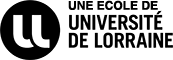
\includegraphics[height=1.25cm]{label-logo-ul.png}}
\ifoot{\noindent\makebox[\linewidth]{\rule{\textwidth}{0.4pt}}\\\textsc{EEIGM - 6, rue Bastien-Lepage - F-54010 Nancy Cedex}}

%\ohead{Abstract}
%\setheadtopline{2pt}
\setheadsepline{0.5pt}
%\setfootsepline{0.5pt}

%\begin{center}
%
%\vspace*{2cm}
%
%\begin{Large}
%\textbf{\textsc{EEIGM}}\\[0.75ex]
%\end{Large}
%
%\begin{large}
%\textbf{\'Ecole Europ\'eenne d'Ing\'enieurs en G\'enie des Mat\'eriaux}\\[0.75ex]
%\end{large}
%
%\vspace{2cm}
%
%\begin{large}
%\textbf{$2^{`eme}$ Ann\'ee, $1^{er}$ Semestre}\\[0.75ex]
%\end{large}
%\vspace*{0.5cm}
%
%\begin{Large}
%\textbf{\textsc{M\'ecanique du Solide D\'eformable}}\\[0.75ex]
%\end{Large}
%\vspace*{0.5cm}
%
%\begin{Large}
%\textbf{\textsc{Travaux Dirig\'es}}\\[0.75ex]
%\end{Large}
%\vspace*{2.5cm}
%
%\begin{large}
%\textbf{Luca Di Stasio}\\[0.75ex]
%\end{large}
%
%\vspace{2cm}
%%\begin{flushright}
%%\begin{tabular}{l l }
%%{\large \textbf{Author(s):}} & {\large Luca DI STASIO}\\
%%\end{tabular}
%%\end{flushright}
%
%\begin{large}
%\ccLogo\ccAttribution\ccNonCommercial\\[0.75ex]
%Cette oeuvre est mise \`a disposition selon les termes de la\\ \href{https://creativecommons.org/licenses/by-nc/4.0/deed.fr}{Licence Creative Commons Attribution - Pas d'Utilisation Commerciale 4.0 International}.\\[0.75ex]
%\end{large}
%
%\vspace*{3cm}
%
%
%{\large \textbf{\today}}\\
%%\textsc{DEFENSE LOCATION}\\
%
%%------------------------------------------------
%% Committee members:
%%\textbf{\textsc{Committee Members}}\\[0.75ex]
%%\textsc{NAME AND AFFILIATION}\\
%%\textsc{NAME AND AFFILIATION}\\
%%\textsc{NAME AND AFFILIATION}\\
%%\textsc{ }\\
%
%\end{center}

%\newpage

%------------------------------------------------%
%            Table of Contents
%------------------------------------------------%

%\pagenumbering{roman}
%
%\setcounter{page}{1}
%
%\clearscrheadings
%\pagestyle{scrheadings}
%\manualmark
%\ofoot{\\ \pagemark} % ofoo
%\ifoot{} % ofoo
%%\cfoot[]{\pagemark}
%%\ihead{}
%%\ohead{}
%\ohead{Table des mati\`eres}
%\setheadtopline{2pt}
%\setheadsepline{0.5pt}
%\setfootsepline{0.5pt}
%
%\hypertarget{contents}{}
%\tableofcontents 
%
%\cleardoublepage

%------------------------------------------------%
%            List of Acronyms
%------------------------------------------------%

%\clearscrheadings
%\pagestyle{scrheadings}
%\manualmark
%\ofoot{\\ \pagemark} % ofoo
%\ifoot{} % ofoo
%%\cfoot[]{\pagemark}
%%\ihead{}
%%\ohead{}
%\ohead{List of Acronyms}
%\setheadtopline{2pt}
%\setheadsepline{0.5pt}
%\setfootsepline{0.5pt}
%
%\section*{List of Acronyms}
%\addcontentsline{toc}{section}{List of Acronyms}
%
%\cleardoublepageusingstyle{scrheadings}

%------------------------------------------------%
%            List of Symbols
%------------------------------------------------%

%\clearscrheadings
%\pagestyle{scrheadings}
%\manualmark
%\ofoot{\\ \pagemark} % ofoo
%\ifoot{} % ofoo
%%\cfoot[]{\pagemark}
%%\ihead{}
%%\ohead{}
%\ohead{List of Symbols}
%\setheadtopline{2pt}
%\setheadsepline{0.5pt}
%\setfootsepline{0.5pt}
%
%\section*{List of Symbols}
%\addcontentsline{toc}{section}{List of Symbols}
%
%\cleardoublepageusingstyle{scrheadings}

%------------------------------------------------%
%                       Abstract
%------------------------------------------------%

%\clearscrheadings
%\pagestyle{scrheadings}
%\manualmark
%\ofoot{\\ \pagemark} % ofoo
%\ifoot{} % ofoo
%%\cfoot[]{\pagemark}
%%\ihead{}
%%\ohead{}
%\ohead{Abstract}
%\setheadtopline{2pt}
%\setheadsepline{0.5pt}
%\setfootsepline{0.5pt}
%
%\section*{Abstract}
%\addcontentsline{toc}{section}{Abstract}
%
%\cleardoublepageusingstyle{scrheadings}

%------------------------------------------------%
%------------------------------------------------%
%                   Main Matter                          %
%------------------------------------------------%
%------------------------------------------------%

\pagenumbering{arabic}

\setcounter{page}{1}

%----------------------------------------------------------------------%
%                   Systemes de coordonnees curvilignes
%----------------------------------------------------------------------%

\clearscrheadings
\pagestyle{scrheadings}
\manualmark
\ofoot{\\\pagemark} % ofoo
%\ifoot{\hyperlink{contents}{Retourner \'a la table des mati\`eres}} % ofoo
\ifoot{}
%\cfoot[]{\pagemark}
\ihead{}
%\ohead{}
%\ihead{\hyperlink{contents}{Retourner \'a la table des mati\`eres}}
\ohead{TD 3 (BONUS)}
\setheadtopline{2pt}
\setheadsepline{0.5pt}
\setfootsepline{0.5pt}

\section*{Exercice optionnel TD 3}

%\subsection{\'Enonc\'e}
%
%\subsubsection{Probl\`eme A}
%
%D\'eterminer l'expression de
%
%\begin{itemize}
%\renewcommand\labelitemi{--}
%\item les vecteurs du rep\`ere local naturel (base covariante),
%\item le jacobien de la transformation,
%\item le tenseur m\'etrique,
%\item le d\'eplacement infinit\'esimal d'un point,
%\item l'\'el\'ement infinit\'esimal de ligne,
%\item l'\'el\'ement infinit\'esimal de volume;
%\end{itemize}
%
%dans un syst\`eme de coordonn\'ees
%
%\begin{enumerate}
%\item cylindriques,
%\item sph\'eriques.
%\end{enumerate}
%
%\subsubsection{Probl\`eme B}
%
%Exprimer l'op\'erateur laplacien $\nabla^{2}$ en
%
%\begin{enumerate}
%\item coordonn\'ees cylindriques,
%\item coordonn\'ees spheriques.
%\end{enumerate}
%
%\subsubsection{Probl\`eme C}
%
%D\'eriver l'expression des vecteurs de la base contravariante et du gradient d'un fonction scalaire $\nabla f$ en
%
%\begin{enumerate}
%\item coordonn\'ees cylindriques,
%\item coordonn\'ees spheriques.
%\end{enumerate}
%
%\newpage
%
%\subsection{Corrig\'e}
%
%\subsubsection{Probl\`eme A}
%
%\begin{description}
%
%\item[Rappels th\'eoriques]
%
%\begin{equation}
%\begin{cases}
%x=x\left(\xi,\eta,\zeta\right)\\
%y=y\left(\xi,\eta,\zeta\right)\\
%z=z\left(\xi,\eta,\zeta\right)
%\end{cases}\longleftrightarrow\begin{cases}
%\xi=\xi\left(x,y,z\right)\\
%\eta=\eta\left(x,y,z\right)\\
%\zeta=\zeta\left(x,y,z\right)
%\end{cases}
%\end{equation}
%
%\begin{equation}
%\mathbf{r}=\begin{bmatrix}
%x\\
%y\\
%z\\
%\end{bmatrix}=\begin{bmatrix}
%\xi\\
%\eta\\
%\zeta\\
%\end{bmatrix}
%\end{equation}
%
%\begin{equation}
%d\mathbf{r}=\begin{bmatrix}
%dx\\
%dy\\
%dz\\
%\end{bmatrix}
%\end{equation}
%
%\begin{equation}
%\begin{cases}
%dx=\frac{\partial x}{\partial\xi}d \xi+\frac{\partial x}{\partial\eta}d \eta+\frac{\partial x}{\partial\zeta}d \zeta\\
%dy=\frac{\partial y}{\partial\xi}d \xi+\frac{\partial y}{\partial\eta}d \eta+\frac{\partial y}{\partial\zeta}d \zeta\\
%dz=\frac{\partial z}{\partial\xi}d \xi+\frac{\partial z}{\partial\eta}d \eta+\frac{\partial z}{\partial\zeta}d \zeta\\
%\end{cases}
%\end{equation}
%
%\begin{equation}
%d\mathbf{r}=\begin{bmatrix}
%dx\\
%dy\\
%dz\\
%\end{bmatrix}=\underbrace{\begin{bmatrix}
%\frac{\partial x}{\partial\xi}&\frac{\partial x}{\partial\eta}&\frac{\partial x}{\partial\zeta}\\
%\frac{\partial y}{\partial\xi}&\frac{\partial y}{\partial\eta}&\frac{\partial y}{\partial\zeta}\\
%\frac{\partial z}{\partial\xi}&\frac{\partial z}{\partial\eta}&\frac{\partial z}{\partial\zeta}\\
%\end{bmatrix}}_{\mathbf{J}}\begin{bmatrix}
%d\xi\\
%d\eta\\
%d\zeta\\
%\end{bmatrix}=\mathbf{J}\begin{bmatrix}
%d\xi\\
%d\eta\\
%d\zeta\\
%\end{bmatrix}
%\end{equation}
%
%\tikzset{node style ge/.style={circle}}
%
%\begin{center}
%\begin{tabular}{ccc}
%\begin{tikzpicture}
%\matrix (A) [matrix of math nodes,left delimiter={[},right delimiter={]}] 
%{ \frac{\partial x}{\partial\xi}&\frac{\partial x}{\partial\eta}&\frac{\partial x}{\partial\zeta}\\
%\frac{\partial y}{\partial\xi}&\frac{\partial y}{\partial\eta}&\frac{\partial y}{\partial\zeta}\\
%\frac{\partial z}{\partial\xi}&\frac{\partial z}{\partial\eta}&\frac{\partial z}{\partial\zeta}\\
%};
%\draw [blue!50!black,fill=blue!10!white,fill opacity =0.25] (A-1-1.north east) to (A-3-1.south east) to (A-3-1.south west) to (A-1-1.north west) to (A-1-1.north east);
%\end{tikzpicture}
%&
%\begin{tikzpicture}
%\matrix (A) [matrix of math nodes,left delimiter={[},right delimiter={]}] 
%{ \frac{\partial x}{\partial\xi}&\frac{\partial x}{\partial\eta}&\frac{\partial x}{\partial\zeta}\\
%\frac{\partial y}{\partial\xi}&\frac{\partial y}{\partial\eta}&\frac{\partial y}{\partial\zeta}\\
%\frac{\partial z}{\partial\xi}&\frac{\partial z}{\partial\eta}&\frac{\partial z}{\partial\zeta}\\
%};
%\draw [green!30!black,fill=green!10!white,fill opacity =0.25] (A-1-2.north east) to (A-3-2.south east) to (A-3-2.south west) to (A-1-2.north west) to (A-1-2.north east);
%\end{tikzpicture}
%&
%\begin{tikzpicture}
%\matrix (A) [matrix of math nodes,left delimiter={[},right delimiter={]}] 
%{ \frac{\partial x}{\partial\xi}&\frac{\partial x}{\partial\eta}&\frac{\partial x}{\partial\zeta}\\
%\frac{\partial y}{\partial\xi}&\frac{\partial y}{\partial\eta}&\frac{\partial y}{\partial\zeta}\\
%\frac{\partial z}{\partial\xi}&\frac{\partial z}{\partial\eta}&\frac{\partial z}{\partial\zeta}\\
%};
%\draw [purple!50!black,fill=purple!10!white,fill opacity =0.25] (A-1-3.north east) to (A-3-3.south east) to (A-3-3.south west) to (A-1-3.north west) to (A-1-3.north east);
%\end{tikzpicture}
%\\
%$\color{blue!50!black} \frac{\partial \mathbf{r}}{\partial\xi}$&$\color{green!30!black} \frac{\partial \mathbf{r}}{\partial\eta}$&$\color{purple!50!black} \frac{\partial \mathbf{r}}{\partial\zeta}$\\
%\end{tabular}
%\end{center}
%
%\begin{equation}
%\begin{aligned}
%\mathbf{i}_{\xi}=&\frac{1}{\lvert\lvert\frac{\partial \mathbf{r}}{\partial\xi}\rvert\rvert}\frac{\partial \mathbf{r}}{\partial\xi}=\frac{1}{\sqrt{\left(\frac{\partial x}{\partial\xi}\right)^{2}+\left(\frac{\partial y}{\partial\xi}\right)^{2}+\left(\frac{\partial z}{\partial\xi}\right)^{2}}}\begin{bmatrix}
%\frac{\partial x}{\partial\xi}\\[5pt]
%\frac{\partial y}{\partial\xi}\\[5pt]
%\frac{\partial z}{\partial\xi}\end{bmatrix}\\
%\mathbf{j}_{\eta}=&\frac{1}{\lvert\lvert\frac{\partial \mathbf{r}}{\partial\eta}\rvert\rvert}\frac{\partial \mathbf{r}}{\partial\eta}=\frac{1}{\sqrt{\left(\frac{\partial x}{\partial\eta}\right)^{2}+\left(\frac{\partial y}{\partial\eta}\right)^{2}+\left(\frac{\partial z}{\partial\eta}\right)^{2}}}\begin{bmatrix}
%\frac{\partial x}{\partial\eta}\\[5pt]
%\frac{\partial y}{\partial\eta}\\[5pt]
%\frac{\partial z}{\partial\eta}\end{bmatrix}\\
%\mathbf{k}_{\zeta}=&\frac{1}{\lvert\lvert\frac{\partial \mathbf{r}}{\partial\zeta}\rvert\rvert}\frac{\partial \mathbf{r}}{\partial\zeta}=\frac{1}{\sqrt{\left(\frac{\partial x}{\partial\zeta}\right)^{2}+\left(\frac{\partial y}{\partial\zeta}\right)^{2}+\left(\frac{\partial z}{\partial\zeta}\right)^{2}}}\begin{bmatrix}
%\frac{\partial x}{\partial\zeta}\\[5pt]
%\frac{\partial y}{\partial\zeta}\\[5pt]
%\frac{\partial z}{\partial\zeta}\end{bmatrix}
%\end{aligned}
%\end{equation}
%
%\begin{equation}
%dl^{2}=d\mathbf{r}^{T}d\mathbf{r}=\begin{bmatrix}
%dx&
%dy&
%dz\\
%\end{bmatrix}\begin{bmatrix}
%dx\\
%dy\\
%dz\\
%\end{bmatrix}=dx^{2}+dy^{2}+dz^{2}
%\end{equation}
%
%\begin{equation}
%\footnotesize
%\begin{aligned}
%dl^{2}&=d\mathbf{r}^{T}d\mathbf{r}=\begin{bmatrix}
%d\xi&
%d\eta&
%d\zeta\\
%\end{bmatrix}\mathbf{J}^{T}\mathbf{J}\begin{bmatrix}
%d\xi\\
%d\eta\\
%d\zeta\\
%\end{bmatrix}=\\&=\begin{bmatrix}
%d\xi&
%d\eta&
%d\zeta\\
%\end{bmatrix}\begin{bmatrix}
%\frac{\partial x}{\partial\xi}&\frac{\partial y}{\partial\xi}&\frac{\partial z}{\partial\xi}\\
%\frac{\partial x}{\partial\eta}&\frac{\partial y}{\partial\eta}&\frac{\partial z}{\partial\eta}\\
%\frac{\partial x}{\partial\zeta}&\frac{\partial y}{\partial\zeta}&\frac{\partial z}{\partial\zeta}\\
%\end{bmatrix}\begin{bmatrix}
%\frac{\partial x}{\partial\xi}&\frac{\partial x}{\partial\eta}&\frac{\partial x}{\partial\zeta}\\
%\frac{\partial y}{\partial\xi}&\frac{\partial y}{\partial\eta}&\frac{\partial y}{\partial\zeta}\\
%\frac{\partial z}{\partial\xi}&\frac{\partial z}{\partial\eta}&\frac{\partial z}{\partial\zeta}\\
%\end{bmatrix}\begin{bmatrix}
%d\xi\\
%d\eta\\
%d\zeta\\
%\end{bmatrix}=\\&=\begin{bmatrix}
%d\xi&
%d\eta&
%d\zeta\\
%\end{bmatrix}\underbrace{\begin{bmatrix}
%\left(\frac{\partial x}{\partial\xi}\right)^{2}+\left(\frac{\partial y}{\partial\xi}\right)^{2}+\left(\frac{\partial z}{\partial\xi}\right)^{2}&\frac{\partial x}{\partial\xi}\frac{\partial x}{\partial\eta}+\frac{\partial y}{\partial\xi}\frac{\partial y}{\partial\eta}+\frac{\partial z}{\partial\xi}\frac{\partial z}{\partial\eta}&\frac{\partial x}{\partial\xi}\frac{\partial x}{\partial\zeta}+\frac{\partial y}{\partial\xi}\frac{\partial y}{\partial\zeta}+\frac{\partial z}{\partial\xi}\frac{\partial z}{\partial\zeta}\\
%\frac{\partial x}{\partial\xi}\frac{\partial x}{\partial\eta}+\frac{\partial y}{\partial\xi}\frac{\partial y}{\partial\eta}+\frac{\partial z}{\partial\xi}\frac{\partial z}{\partial\eta}&\left(\frac{\partial x}{\partial\eta}\right)^{2}+\left(\frac{\partial y}{\partial\eta}\right)^{2}+\left(\frac{\partial z}{\partial\eta}\right)^{2}&\frac{\partial x}{\partial\eta}\frac{\partial x}{\partial\zeta}+\frac{\partial y}{\partial\eta}\frac{\partial y}{\partial\zeta}+\frac{\partial z}{\partial\eta}\frac{\partial z}{\partial\zeta}\\
%\frac{\partial x}{\partial\xi}\frac{\partial x}{\partial\zeta}+\frac{\partial y}{\partial\xi}\frac{\partial y}{\partial\zeta}+\frac{\partial z}{\partial\xi}\frac{\partial z}{\partial\zeta}&\frac{\partial x}{\partial\eta}\frac{\partial x}{\partial\zeta}+\frac{\partial y}{\partial\eta}\frac{\partial y}{\partial\zeta}+\frac{\partial z}{\partial\eta}\frac{\partial z}{\partial\zeta}&\left(\frac{\partial x}{\partial\zeta}\right)^{2}+\left(\frac{\partial y}{\partial\zeta}\right)^{2}+\left(\frac{\partial z}{\partial\zeta}\right)^{2}\\
%\end{bmatrix}}_{\mathbf{g}}\begin{bmatrix}
%d\xi\\
%d\eta\\
%d\zeta\\
%\end{bmatrix}
%\end{aligned}
%\end{equation}
%
%\begin{equation}
%dV=\frac{\partial \mathbf{r}}{\partial\xi}d\xi\cdot\left(\frac{\partial \mathbf{r}}{\partial\eta}d\eta\wedge\frac{\partial \mathbf{r}}{\partial\zeta}d\zeta\right)=det\begin{bmatrix}
%\left(\frac{\partial \mathbf{r}}{\partial\xi}\right)^{T}\\
%\left(\frac{\partial \mathbf{r}}{\partial\eta}\right)^{T}\\
%\left(\frac{\partial \mathbf{r}}{\partial\zeta}\right)^{T}\\
%\end{bmatrix}d\xi d\eta d\zeta=det\left(\mathbf{J}^{T}\right)d\xi d\eta d\zeta
%\end{equation}
%
%\newpage
%
%\item[Coordonn\'ees cylindriques]
%
%\begin{equation}
%\begin{cases}
%x=r\cos{\theta}\\
%y=r\sin{\theta}\\
%z=\tilde{z}
%\end{cases}\longleftrightarrow\begin{cases}
%r=\sqrt{x^{2}+y^{2}}\\
%\theta=\tan^{-1}\left(\frac{y}{x}\right)\\
%\tilde{z}=z
%\end{cases}
%\end{equation}
%
%\begin{equation}
%\begin{cases}
%\frac{\partial x}{\partial r}&=\cos{\theta}\\
%\frac{\partial x}{\partial \theta}&=-r\sin{\theta}\\
%\frac{\partial x}{\partial \tilde{z}}&=0\\
%\end{cases}\qquad\begin{cases}
%\frac{\partial y}{\partial r}&=\sin{\theta}\\
%\frac{\partial y}{\partial \theta}&=r\cos{\theta}\\
%\frac{\partial y}{\partial \tilde{z}}&=0\\
%\end{cases}\qquad\begin{cases}
%\frac{\partial z}{\partial r}&=0\\
%\frac{\partial z}{\partial \theta}&=0\\
%\frac{\partial z}{\partial \tilde{z}}&=1\\
%\end{cases}
%\end{equation}
%
%\begin{equation}
%\begin{aligned}
%\mathbf{i}_{r}=&\frac{1}{\lvert\lvert\frac{\partial \mathbf{r}}{\partial r}\rvert\rvert}\frac{\partial \mathbf{r}}{\partial r}=\frac{1}{\sqrt{\sin^{2}{\theta}+\cos^{2}{\theta}}}\begin{bmatrix}
%\cos{\theta}\\[5pt]
%\sin{\theta}\\[5pt]
%0\end{bmatrix}=\begin{bmatrix}
%\cos{\theta}\\[5pt]
%\sin{\theta}\\[5pt]
%0\end{bmatrix}\\
%\mathbf{j}_{\theta}=&\frac{1}{\lvert\lvert\frac{\partial \mathbf{r}}{\partial\theta}\rvert\rvert}\frac{\partial \mathbf{r}}{\partial\theta}=\frac{1}{\sqrt{r^{2}\sin^{2}{\theta}+r^{2}\cos^{2}{\theta}}}\begin{bmatrix}
%-r\sin{\theta}\\[5pt]
%r\cos{\theta}\\[5pt]
%0\end{bmatrix}=\begin{bmatrix}
%-\sin{\theta}\\[5pt]
%\cos{\theta}\\[5pt]
%0\end{bmatrix}\\
%\mathbf{k}_{\tilde{z}}=&\frac{1}{\lvert\lvert\frac{\partial \mathbf{r}}{\partial\tilde{z}}\rvert\rvert}\frac{\partial \mathbf{r}}{\partial\tilde{z}}=\begin{bmatrix}
%0\\[5pt]
%0\\[5pt]
%1\end{bmatrix}
%\end{aligned}
%\end{equation}
%
%\begin{equation}
%\mathbf{J}=\begin{bmatrix}
%\cos{\theta}&-r\sin{\theta}&0\\
%\sin{\theta}&r\cos{\theta}&0\\
%0&0&1\\
%\end{bmatrix}
%\end{equation}
%
%\begin{equation}
%d\mathbf{r}=\begin{bmatrix}
%\cos{\theta}\\
%\sin{\theta}\\
%0\\
%\end{bmatrix}dr+\begin{bmatrix}
%-r\sin{\theta}\\
%r\cos{\theta}\\
%0\\
%\end{bmatrix}d\theta+\begin{bmatrix}
%0\\
%0\\
%1\\
%\end{bmatrix}d\tilde{z}=dr\mathbf{i}_{r}+rd\theta\mathbf{i}_{\theta}+d\tilde{z}\mathbf{i}_{\tilde{z}}=\begin{bmatrix}
%dr\\
%rd\theta\\
%d\tilde{z}\\
%\end{bmatrix}
%\end{equation}
%
%\begin{equation}
%\mathbf{g}=
%\begin{bmatrix}
%1&0&0\\
%0&r^{2}&0\\
%0&0&1\\
%\end{bmatrix}
%\end{equation}
%
%\begin{equation}
%dl^{2}=dr^{2}+r^{2}d\theta^{2}+d\tilde{z}^{2}
%\end{equation}
%
%\begin{equation}
%dV=det\left(\mathbf{J}^{T}\right)drd\theta d\tilde{z}=rdrd\theta d\tilde{z}
%\end{equation}
%
%\item[Coordonn\'ees spheriques]
%
%\begin{equation}
%\begin{cases}
%x=r\sin{\theta}\cos{\varphi}\\
%y=r\sin{\theta}\sin{\varphi}\\
%z=r\cos{\theta}
%\end{cases}\longleftrightarrow\begin{cases}
%r=\sqrt{x^{2}+y^{2}+z^{2}}\\
%\varphi=\tan^{-1}\left(\frac{y}{x}\right)\\
%\theta=\tan^{-1}\left(\frac{\sqrt{x^{2}+y^{2}}}{z}\right)\\
%\end{cases}
%\end{equation}
%
%\begin{equation}
%\begin{cases}
%\frac{\partial x}{\partial r}&=\sin{\theta}\cos{\varphi}\\
%\frac{\partial x}{\partial \theta}&=r\cos{\theta}\cos{\varphi}\\
%\frac{\partial x}{\partial \varphi}&=-r\sin{\theta}\sin{\varphi}\\
%\end{cases}\qquad\begin{cases}
%\frac{\partial y}{\partial r}&=\sin{\theta}\sin{\varphi}\\
%\frac{\partial y}{\partial \theta}&=r\cos{\theta}\sin{\varphi}\\
%\frac{\partial y}{\partial \varphi}&=r\sin{\theta}\cos{\varphi}\\
%\end{cases}\qquad\begin{cases}
%\frac{\partial z}{\partial r}&=\cos{\theta}\\
%\frac{\partial z}{\partial \theta}&=-r\sin{\theta}\\
%\frac{\partial z}{\partial \varphi}&=0\\
%\end{cases}
%\end{equation}
%
%\begin{equation}
%\begin{aligned}
%\mathbf{i}_{r}=&\frac{1}{\lvert\lvert\frac{\partial \mathbf{r}}{\partial r}\rvert\rvert}\frac{\partial \mathbf{r}}{\partial r}=\frac{1}{\sqrt{\sin^{2}{\theta}\cos^{2}{\varphi}+\sin^{2}{\theta}\sin^{2}{\varphi}+\cos^{2}{\theta}}}\begin{bmatrix}
%\sin{\theta}\cos{\varphi}\\[5pt]
%\sin{\theta}\sin{\varphi}\\[5pt]
%\cos{\theta}\end{bmatrix}=\begin{bmatrix}
%\sin{\theta}\cos{\varphi}\\[5pt]
%\sin{\theta}\sin{\varphi}\\[5pt]
%\cos{\theta}\end{bmatrix}\\
%\mathbf{j}_{\varphi}=&\frac{1}{\lvert\lvert\frac{\partial \mathbf{r}}{\partial\varphi}\rvert\rvert}\frac{\partial \mathbf{r}}{\partial\varphi}=\frac{1}{\sqrt{r^{2}\sin^{2}{\theta}\sin^{2}{\varphi}+r^{2}\sin^{2}{\theta}\cos^{2}{\varphi}}}\begin{bmatrix}
%-r\sin{\theta}\sin{\varphi}\\[5pt]
%r\sin{\theta}\cos{\varphi}\\[5pt]
%0\end{bmatrix}=\begin{bmatrix}
%-\sin{\varphi}\\[5pt]
%\cos{\varphi}\\[5pt]
%0\end{bmatrix}\\
%\mathbf{k}_{\theta}=&\frac{1}{\lvert\lvert\frac{\partial \mathbf{r}}{\partial\theta}\rvert\rvert}\frac{\partial \mathbf{r}}{\partial\theta}=\frac{1}{\sqrt{r^{2}\cos^{2}{\theta}\cos^{2}{\varphi}+r^{2}\cos^{2}{\theta}\sin^{2}{\varphi}+r^{2}\sin^{2}{\theta}}}\begin{bmatrix}
%r\cos{\theta}\cos{\varphi}\\[5pt]
%r\cos{\theta}\sin{\varphi}\\[5pt]
%-r\sin{\theta}\end{bmatrix}=\begin{bmatrix}
%\cos{\theta}\cos{\varphi}\\[5pt]
%\cos{\theta}\sin{\varphi}\\[5pt]
%-\sin{\theta}\end{bmatrix}\\
%\end{aligned}
%\end{equation}
%
%\begin{equation}
%\mathbf{J}=\begin{bmatrix}
%\sin{\theta}\cos{\varphi}&-r\sin{\theta}\sin{\varphi}&r\cos{\theta}\cos{\varphi}\\
%\sin{\theta}\sin{\varphi}&r\sin{\theta}\cos{\varphi}&r\cos{\theta}\sin{\varphi}\\
%\cos{\theta}&0&-r\sin{\theta}\\
%\end{bmatrix}
%\end{equation}
%
%\begin{equation}
%\begin{aligned}
%d\mathbf{r}&=\begin{bmatrix}
%\sin{\theta}\cos{\varphi}\\
%\sin{\theta}\sin{\varphi}\\
%\cos{\theta}\\
%\end{bmatrix}dr+r\sin{\theta}\begin{bmatrix}
%-\sin{\varphi}\\
%\cos{\varphi}\\
%0\\
%\end{bmatrix}d\varphi+r\begin{bmatrix}
%\cos{\theta}\cos{\varphi}\\
%\cos{\theta}\sin{\varphi}\\
%-\sin{\theta}\\
%\end{bmatrix}d\theta=\\
%&=dr\mathbf{i}_{r}+r\sin{\theta}d\varphi\mathbf{j}_{\varphi}+rd\theta\mathbf{k}_{\theta}=\begin{bmatrix}
%dr\\
%r\sin{\theta}d\varphi\\
%rd\theta\\
%\end{bmatrix}
%\end{aligned}
%\end{equation}
%
%\begin{equation}
%\mathbf{g}=
%\begin{bmatrix}
%1&0&0\\
%0&r^{2}\sin^{2}{\theta}&0\\
%0&0&r^{2}\\
%\end{bmatrix}
%\end{equation}
%
%\begin{equation}
%dl^{2}=dr^{2}+r^{2}\sin^{2}{\theta}d\varphi^{2}+r^{2}d\theta^{2}
%\end{equation}
%
%\begin{equation}
%dV=det\left(\mathbf{J}^{T}\right)drd\theta d\tilde{z}=r^{2}\sin{\theta}drd\varphi d\theta
%\end{equation}
%
%\end{description}
%
%\newpage
%
%\subsubsection{Probl\`eme B}
%
%\begin{description}
%
%\item[Rappels th\'eoriques]
%
%\begin{equation}
%\begin{cases}
%x=x\left(\xi,\eta,\zeta\right)\\
%y=y\left(\xi,\eta,\zeta\right)\\
%z=z\left(\xi,\eta,\zeta\right)
%\end{cases}\longleftrightarrow\begin{cases}
%\xi=\xi\left(x,y,z\right)\\
%\eta=\eta\left(x,y,z\right)\\
%\zeta=\zeta\left(x,y,z\right)
%\end{cases}
%\end{equation}
%
%\begin{equation}
%f\left(x,y,z\right)=f\left(x\left(\xi,\eta,\zeta\right),y\left(\xi,\eta,\zeta\right),z\left(\xi,\eta,\zeta\right)\right)
%\end{equation}
%
%\begin{equation}
%f\left(\xi,\eta,\zeta\right)=f\left(\xi\left(x,y,z\right),\eta\left(x,y,z\right),\zeta\left(x,y,z\right)\right)
%\end{equation}
%
%\begin{equation}
%\nabla_{xyz}^{2}f\left(x,y,z\right)=\frac{\partial^{2} f}{\partial x^{2}}+\frac{\partial^{2} f}{\partial y^{2}}+\frac{\partial^{2} f}{\partial z^{2}}
%\end{equation}
%
%\begin{equation}
%\begin{cases}
%\frac{\partial f}{\partial x}=\frac{\partial f}{\partial\xi}\frac{\partial\xi}{\partial x}+\frac{\partial f}{\partial\eta}\frac{\partial\eta}{\partial x}+\frac{\partial f}{\partial\zeta}\frac{\partial\zeta}{\partial x}\\[5pt]
%\frac{\partial f}{\partial y}=\frac{\partial f}{\partial\xi}\frac{\partial\xi}{\partial y}+\frac{\partial f}{\partial\eta}\frac{\partial\eta}{\partial y}+\frac{\partial f}{\partial\zeta}\frac{\partial\zeta}{\partial y}\\[5pt]
%\frac{\partial f}{\partial z}=\frac{\partial f}{\partial\xi}\frac{\partial\xi}{\partial z}+\frac{\partial f}{\partial\eta}\frac{\partial\eta}{\partial z}+\frac{\partial f}{\partial\zeta}\frac{\partial\zeta}{\partial z}
%\end{cases}
%\end{equation}
%
%\begin{equation}
%\begin{cases}
%\frac{\partial^{2} f}{\partial x^{2}}&=\frac{\partial}{\partial x}\left(\frac{\partial f}{\partial\xi}\frac{\partial\xi}{\partial x}+\frac{\partial f}{\partial\eta}\frac{\partial\eta}{\partial x}+\frac{\partial f}{\partial\zeta}\frac{\partial\zeta}{\partial x}\right)=\\[5pt]
%&=\frac{\partial}{\partial x}\left(\frac{\partial f}{\partial\xi}\right)\frac{\partial\xi}{\partial x}+\frac{\partial}{\partial x}\left(\frac{\partial f}{\partial\eta}\right)\frac{\partial\eta}{\partial x}+\frac{\partial}{\partial x}\left(\frac{\partial f}{\partial\zeta}\right)\frac{\partial\zeta}{\partial x}+\frac{\partial f}{\partial\xi}\frac{\partial^{2}\xi}{\partial x^{2}}+\frac{\partial f}{\partial\eta}\frac{\partial^{2}\eta}{\partial x^{2}}+\frac{\partial f}{\partial\zeta}\frac{\partial^{2}\zeta}{\partial x^{2}}\\[10pt]
%%
%\frac{\partial^{2} f}{\partial y^{2}}&=\frac{\partial}{\partial y}\left(\frac{\partial f}{\partial\xi}\frac{\partial\xi}{\partial y}+\frac{\partial f}{\partial\eta}\frac{\partial\eta}{\partial y}+\frac{\partial f}{\partial\zeta}\frac{\partial\zeta}{\partial y}\right)=\\[5pt]
%&=\frac{\partial}{\partial y}\left(\frac{\partial f}{\partial\xi}\right)\frac{\partial\xi}{\partial y}+\frac{\partial}{\partial y}\left(\frac{\partial f}{\partial\eta}\right)\frac{\partial\eta}{\partial y}+\frac{\partial}{\partial y}\left(\frac{\partial f}{\partial\zeta}\right)\frac{\partial\zeta}{\partial y}+\frac{\partial f}{\partial\xi}\frac{\partial^{2}\xi}{\partial y^{2}}+\frac{\partial f}{\partial\eta}\frac{\partial^{2}\eta}{\partial y^{2}}+\frac{\partial f}{\partial\zeta}\frac{\partial^{2}\zeta}{\partial y^{2}}\\[10pt]
%%
%\frac{\partial^{2} f}{\partial z^{2}}&=\frac{\partial}{\partial z}\left(\frac{\partial f}{\partial\xi}\frac{\partial\xi}{\partial z}+\frac{\partial f}{\partial\eta}\frac{\partial\eta}{\partial z}+\frac{\partial f}{\partial\zeta}\frac{\partial\zeta}{\partial z}\right)=\\[5pt]
%&=\frac{\partial}{\partial z}\left(\frac{\partial f}{\partial\xi}\right)\frac{\partial\xi}{\partial z}+\frac{\partial}{\partial z}\left(\frac{\partial f}{\partial\eta}\right)\frac{\partial\eta}{\partial z}+\frac{\partial}{\partial z}\left(\frac{\partial f}{\partial\zeta}\right)\frac{\partial\zeta}{\partial z}+\frac{\partial f}{\partial\xi}\frac{\partial^{2}\xi}{\partial z^{2}}+\frac{\partial f}{\partial\eta}\frac{\partial^{2}\eta}{\partial z^{2}}+\frac{\partial f}{\partial\zeta}\frac{\partial^{2}\zeta}{\partial z^{2}}\\[10pt]
%\end{cases}
%\end{equation}
%
%\begin{equation}
%\begin{cases}
%\frac{\partial}{\partial x}=\left(\frac{\partial\xi}{\partial x}\frac{\partial}{\partial\xi}+\frac{\partial\eta}{\partial x}\frac{\partial}{\partial\eta}+\frac{\partial\zeta}{\partial x}\frac{\partial}{\partial\zeta}\right)\\[5pt]
%\frac{\partial}{\partial y}=\left(\frac{\partial\xi}{\partial y}\frac{\partial}{\partial\xi}+\frac{\partial\eta}{\partial y}\frac{\partial}{\partial\eta}+\frac{\partial\zeta}{\partial y}\frac{\partial}{\partial\zeta}\right)\\[5pt]
%\frac{\partial}{\partial z}=\left(\frac{\partial\xi}{\partial z}\frac{\partial}{\partial\xi}+\frac{\partial\eta}{\partial z}\frac{\partial}{\partial\eta}+\frac{\partial\zeta}{\partial z}\frac{\partial}{\partial\zeta}\right)
%\end{cases}
%\end{equation}
%
%\begin{equation}
%\begin{cases}
%\frac{\partial}{\partial x}\left(\frac{\partial f}{\partial\xi}\right)\frac{\partial\xi}{\partial x}&=\left(\frac{\partial\xi}{\partial x}\frac{\partial}{\partial\xi}+\frac{\partial\eta}{\partial x}\frac{\partial}{\partial\eta}+\frac{\partial\zeta}{\partial x}\frac{\partial}{\partial\zeta}\right)\left(\frac{\partial f}{\partial\xi}\right)\frac{\partial\xi}{\partial x}=\\[5pt]
%&=\left(\frac{\partial\xi}{\partial x}\right)^{2}\frac{\partial^{2} f}{\partial\xi^{2}}+\left(\frac{\partial\eta}{\partial x}\right)\left(\frac{\partial\xi}{\partial x}\right)\frac{\partial^{2} f}{\partial\eta\partial\xi}+\left(\frac{\partial\zeta}{\partial x}\right)\left(\frac{\partial\xi}{\partial x}\right)\frac{\partial^{2} f}{\partial\zeta\partial\xi}\\[10pt]
%\frac{\partial}{\partial x}\left(\frac{\partial f}{\partial\eta}\right)\frac{\partial\eta}{\partial x}&=\left(\frac{\partial\xi}{\partial x}\frac{\partial}{\partial\xi}+\frac{\partial\eta}{\partial x}\frac{\partial}{\partial\eta}+\frac{\partial\zeta}{\partial x}\frac{\partial}{\partial\zeta}\right)\left(\frac{\partial f}{\partial\eta}\right)\frac{\partial\eta}{\partial x}=\\[5pt]
%&=\left(\frac{\partial\xi}{\partial x}\right)\left(\frac{\partial\eta}{\partial x}\right)\frac{\partial^{2} f}{\partial\xi\partial\eta}+\left(\frac{\partial\eta}{\partial x}\right)^{2}\frac{\partial^{2} f}{\partial\eta^{2}}+\left(\frac{\partial\zeta}{\partial x}\right)\left(\frac{\partial\eta}{\partial x}\right)\frac{\partial^{2} f}{\partial\zeta\partial\eta}\\[10pt]
%\frac{\partial}{\partial x}\left(\frac{\partial f}{\partial\zeta}\right)\frac{\partial\zeta}{\partial x}&=\left(\frac{\partial\xi}{\partial x}\frac{\partial}{\partial\xi}+\frac{\partial\eta}{\partial x}\frac{\partial}{\partial\eta}+\frac{\partial\zeta}{\partial x}\frac{\partial}{\partial\zeta}\right)\left(\frac{\partial f}{\partial\zeta}\right)\frac{\partial\zeta}{\partial x}=\\[5pt]
%&=\left(\frac{\partial\xi}{\partial x}\right)\left(\frac{\partial\zeta}{\partial x}\right)\frac{\partial^{2} f}{\partial\xi\partial\zeta}+\left(\frac{\partial\eta}{\partial x}\right)\left(\frac{\partial\zeta}{\partial x}\right)\frac{\partial^{2} f}{\partial\eta\partial\zeta}+\left(\frac{\partial\zeta}{\partial x}\right)^{2}\frac{\partial^{2} f}{\partial\zeta^{2}}\\[5pt]
%\end{cases}
%\end{equation}
%
%\begin{equation}
%\begin{cases}
%\frac{\partial}{\partial y}\left(\frac{\partial f}{\partial\xi}\right)\frac{\partial\xi}{\partial y}&=\left(\frac{\partial\xi}{\partial y}\frac{\partial}{\partial\xi}+\frac{\partial\eta}{\partial y}\frac{\partial}{\partial\eta}+\frac{\partial\zeta}{\partial y}\frac{\partial}{\partial\zeta}\right)\left(\frac{\partial f}{\partial\xi}\right)\frac{\partial\xi}{\partial y}=\\[5pt]
%&=\left(\frac{\partial\xi}{\partial y}\right)^{2}\frac{\partial^{2} f}{\partial\xi^{2}}+\left(\frac{\partial\eta}{\partial y}\right)\left(\frac{\partial\xi}{\partial y}\right)\frac{\partial^{2} f}{\partial\eta\partial\xi}+\left(\frac{\partial\zeta}{\partial y}\right)\left(\frac{\partial\xi}{\partial y}\right)\frac{\partial^{2} f}{\partial\zeta\partial\xi}\\[10pt]
%\frac{\partial}{\partial y}\left(\frac{\partial f}{\partial\eta}\right)\frac{\partial\eta}{\partial y}&=\left(\frac{\partial\xi}{\partial y}\frac{\partial}{\partial\xi}+\frac{\partial\eta}{\partial y}\frac{\partial}{\partial\eta}+\frac{\partial\zeta}{\partial y}\frac{\partial}{\partial\zeta}\right)\left(\frac{\partial f}{\partial\eta}\right)\frac{\partial\eta}{\partial y}=\\[5pt]
%&=\left(\frac{\partial\xi}{\partial y}\right)\left(\frac{\partial\eta}{\partial y}\right)\frac{\partial^{2} f}{\partial\xi\partial\eta}+\left(\frac{\partial\eta}{\partial y}\right)^{2}\frac{\partial^{2} f}{\partial\eta^{2}}+\left(\frac{\partial\zeta}{\partial y}\right)\left(\frac{\partial\eta}{\partial y}\right)\frac{\partial^{2} f}{\partial\zeta\partial\eta}\\[10pt]
%\frac{\partial}{\partial y}\left(\frac{\partial f}{\partial\zeta}\right)\frac{\partial\zeta}{\partial y}&=\left(\frac{\partial\xi}{\partial y}\frac{\partial}{\partial\xi}+\frac{\partial\eta}{\partial y}\frac{\partial}{\partial\eta}+\frac{\partial\zeta}{\partial y}\frac{\partial}{\partial\zeta}\right)\left(\frac{\partial f}{\partial\zeta}\right)\frac{\partial\zeta}{\partial y}=\\[5pt]
%&=\left(\frac{\partial\xi}{\partial y}\right)\left(\frac{\partial\zeta}{\partial y}\right)\frac{\partial^{2} f}{\partial\xi\partial\zeta}+\left(\frac{\partial\eta}{\partial y}\right)\left(\frac{\partial\zeta}{\partial y}\right)\frac{\partial^{2} f}{\partial\eta\partial\zeta}+\left(\frac{\partial\zeta}{\partial y}\right)^{2}\frac{\partial^{2} f}{\partial\zeta^{2}}\\[5pt]
%\end{cases}
%\end{equation}
%
%\begin{equation}
%\begin{cases}
%\frac{\partial}{\partial z}\left(\frac{\partial f}{\partial\xi}\right)\frac{\partial\xi}{\partial z}&=\left(\frac{\partial\xi}{\partial z}\frac{\partial}{\partial\xi}+\frac{\partial\eta}{\partial z}\frac{\partial}{\partial\eta}+\frac{\partial\zeta}{\partial z}\frac{\partial}{\partial\zeta}\right)\left(\frac{\partial f}{\partial\xi}\right)\frac{\partial\xi}{\partial z}=\\[5pt]
%&=\left(\frac{\partial\xi}{\partial z}\right)^{2}\frac{\partial^{2} f}{\partial\xi^{2}}+\left(\frac{\partial\eta}{\partial z}\right)\left(\frac{\partial\xi}{\partial z}\right)\frac{\partial^{2} f}{\partial\eta\partial\xi}+\left(\frac{\partial\zeta}{\partial z}\right)\left(\frac{\partial\xi}{\partial z}\right)\frac{\partial^{2} f}{\partial\zeta\partial\xi}\\[10pt]
%\frac{\partial}{\partial z}\left(\frac{\partial f}{\partial\eta}\right)\frac{\partial\eta}{\partial z}&=\left(\frac{\partial\xi}{\partial z}\frac{\partial}{\partial\xi}+\frac{\partial\eta}{\partial z}\frac{\partial}{\partial\eta}+\frac{\partial\zeta}{\partial z}\frac{\partial}{\partial\zeta}\right)\left(\frac{\partial f}{\partial\eta}\right)\frac{\partial\eta}{\partial z}=\\[5pt]
%&=\left(\frac{\partial\xi}{\partial x}\right)\left(\frac{\partial\eta}{\partial z}\right)\frac{\partial^{2} f}{\partial\xi\partial\eta}+\left(\frac{\partial\eta}{\partial z}\right)^{2}\frac{\partial^{2} f}{\partial\eta^{2}}+\left(\frac{\partial\zeta}{\partial z}\right)\left(\frac{\partial\eta}{\partial z}\right)\frac{\partial^{2} f}{\partial\zeta\partial\eta}\\[10pt]
%\frac{\partial}{\partial z}\left(\frac{\partial f}{\partial\zeta}\right)\frac{\partial\zeta}{\partial z}&=\left(\frac{\partial\xi}{\partial z}\frac{\partial}{\partial\xi}+\frac{\partial\eta}{\partial z}\frac{\partial}{\partial\eta}+\frac{\partial\zeta}{\partial z}\frac{\partial}{\partial\zeta}\right)\left(\frac{\partial f}{\partial\zeta}\right)\frac{\partial\zeta}{\partial z}=\\[5pt]
%&=\left(\frac{\partial\xi}{\partial z}\right)\left(\frac{\partial\zeta}{\partial z}\right)\frac{\partial^{2} f}{\partial\xi\partial\zeta}+\left(\frac{\partial\eta}{\partial z}\right)\left(\frac{\partial\zeta}{\partial z}\right)\frac{\partial^{2} f}{\partial\eta\partial\zeta}+\left(\frac{\partial\zeta}{\partial z}\right)^{2}\frac{\partial^{2} f}{\partial\zeta^{2}}\\[5pt]
%\end{cases}
%\end{equation}
%
%\begin{equation}
%\frac{\partial^{2} f}{\partial\eta\partial\xi}=\frac{\partial^{2} f}{\partial\xi\partial\eta}\qquad\frac{\partial^{2} f}{\partial\eta\partial\zeta}=\frac{\partial^{2} f}{\partial\zeta\partial\eta}\qquad\frac{\partial^{2} f}{\partial\xi\partial\zeta}=\frac{\partial^{2} f}{\partial\zeta\partial\xi}
%\end{equation}
%
%\begin{equation}
%\begin{aligned}
%\frac{\partial^{2} f}{\partial x^{2}}&=\left(\frac{\partial\xi}{\partial x}\right)^{2}\frac{\partial^{2} f}{\partial\xi^{2}}+\left(\frac{\partial\eta}{\partial x}\right)^{2}\frac{\partial^{2} f}{\partial\eta^{2}}+\left(\frac{\partial\zeta}{\partial x}\right)^{2}\frac{\partial^{2} f}{\partial\zeta^{2}}+\\[5pt]
%&+2\left(\frac{\partial\xi}{\partial x}\right)\left(\frac{\partial\eta}{\partial x}\right)\frac{\partial^{2} f}{\partial\xi\partial\eta}+2\left(\frac{\partial\xi}{\partial x}\right)\left(\frac{\partial\zeta}{\partial x}\right)\frac{\partial^{2} f}{\partial\xi\partial\zeta}+2\left(\frac{\partial\eta}{\partial x}\right)\left(\frac{\partial\zeta}{\partial x}\right)\frac{\partial^{2} f}{\partial\eta\partial\zeta}+\\[5pt]
%&+\frac{\partial f}{\partial\xi}\frac{\partial^{2}\xi}{\partial x^{2}}+\frac{\partial f}{\partial\eta}\frac{\partial^{2}\eta}{\partial x^{2}}+\frac{\partial f}{\partial\zeta}\frac{\partial^{2}\zeta}{\partial x^{2}}\\
%\end{aligned}
%\end{equation}
%
%\begin{equation}
%\begin{aligned}
%\frac{\partial^{2} f}{\partial y^{2}}&=\left(\frac{\partial\xi}{\partial y}\right)^{2}\frac{\partial^{2} f}{\partial\xi^{2}}+\left(\frac{\partial\eta}{\partial y}\right)^{2}\frac{\partial^{2} f}{\partial\eta^{2}}+\left(\frac{\partial\zeta}{\partial y}\right)^{2}\frac{\partial^{2} f}{\partial\zeta^{2}}+\\[5pt]
%&+2\left(\frac{\partial\xi}{\partial y}\right)\left(\frac{\partial\eta}{\partial y}\right)\frac{\partial^{2} f}{\partial\xi\partial\eta}+2\left(\frac{\partial\xi}{\partial y}\right)\left(\frac{\partial\zeta}{\partial y}\right)\frac{\partial^{2} f}{\partial\xi\partial\zeta}+2\left(\frac{\partial\eta}{\partial x}\right)\left(\frac{\partial\zeta}{\partial y}\right)\frac{\partial^{2} f}{\partial\eta\partial\zeta}+\\[5pt]
%&+\frac{\partial f}{\partial\xi}\frac{\partial^{2}\xi}{\partial y^{2}}+\frac{\partial f}{\partial\eta}\frac{\partial^{2}\eta}{\partial y^{2}}+\frac{\partial f}{\partial\zeta}\frac{\partial^{2}\zeta}{\partial y^{2}}\\
%\end{aligned}
%\end{equation}
%
%\begin{equation}
%\begin{aligned}
%\frac{\partial^{2} f}{\partial z^{2}}&=\left(\frac{\partial\xi}{\partial z}\right)^{2}\frac{\partial^{2} f}{\partial\xi^{2}}+\left(\frac{\partial\eta}{\partial z}\right)^{2}\frac{\partial^{2} f}{\partial\eta^{2}}+\left(\frac{\partial\zeta}{\partial z}\right)^{2}\frac{\partial^{2} f}{\partial\zeta^{2}}+\\[5pt]
%&+2\left(\frac{\partial\xi}{\partial z}\right)\left(\frac{\partial\eta}{\partial z}\right)\frac{\partial^{2} f}{\partial\xi\partial\eta}+2\left(\frac{\partial\xi}{\partial z}\right)\left(\frac{\partial\zeta}{\partial z}\right)\frac{\partial^{2} f}{\partial\xi\partial\zeta}+2\left(\frac{\partial\eta}{\partial z}\right)\left(\frac{\partial\zeta}{\partial z}\right)\frac{\partial^{2} f}{\partial\eta\partial\zeta}+\\[5pt]
%&+\frac{\partial f}{\partial\xi}\frac{\partial^{2}\xi}{\partial z^{2}}+\frac{\partial f}{\partial\eta}\frac{\partial^{2}\eta}{\partial z^{2}}+\frac{\partial f}{\partial\zeta}\frac{\partial^{2}\zeta}{\partial z^{2}}\\
%\end{aligned}
%\end{equation}
%
%\begin{equation}
%\begin{aligned}
%\nabla_{\xi\eta\zeta}^{2}f\left(\xi,\eta,\zeta\right)=&\left[\left(\frac{\partial\xi}{\partial x}\right)^{2}+\left(\frac{\partial\xi}{\partial y}\right)^{2}+\left(\frac{\partial\xi}{\partial z}\right)^{2}\right]\frac{\partial^{2} f}{\partial\xi^{2}}+\\[5pt]
%&+\left[\left(\frac{\partial\eta}{\partial x}\right)^{2}+\left(\frac{\partial\eta}{\partial y}\right)^{2}+\left(\frac{\partial\eta}{\partial z}\right)^{2}\right]\frac{\partial^{2} f}{\partial\eta^{2}}+\\[5pt]
%&+\left[\left(\frac{\partial\zeta}{\partial x}\right)^{2}+\left(\frac{\partial\zeta}{\partial y}\right)^{2}+\left(\frac{\partial\zeta}{\partial z}\right)^{2}\right]\frac{\partial^{2} f}{\partial\zeta^{2}}+\\[5pt]
%&+2\left[\left(\frac{\partial\xi}{\partial x}\right)\left(\frac{\partial\eta}{\partial x}\right)+\left(\frac{\partial\xi}{\partial y}\right)\left(\frac{\partial\eta}{\partial y}\right)+\left(\frac{\partial\xi}{\partial z}\right)\left(\frac{\partial\eta}{\partial z}\right)\right]\frac{\partial^{2} f}{\partial\xi\partial\eta}+\\[5pt]
%&+2\left[\left(\frac{\partial\eta}{\partial x}\right)\left(\frac{\partial\zeta}{\partial x}\right)+\left(\frac{\partial\eta}{\partial y}\right)\left(\frac{\partial\zeta}{\partial y}\right)+\left(\frac{\partial\eta}{\partial z}\right)\left(\frac{\partial\zeta}{\partial z}\right)\right]\frac{\partial^{2} f}{\partial\eta\partial\zeta}+\\[5pt]
%&+2\left[\left(\frac{\partial\xi}{\partial x}\right)\left(\frac{\partial\zeta}{\partial x}\right)+\left(\frac{\partial\xi}{\partial y}\right)\left(\frac{\partial\zeta}{\partial y}\right)+\left(\frac{\partial\xi}{\partial z}\right)\left(\frac{\partial\zeta}{\partial z}\right)\right]\frac{\partial^{2} f}{\partial\xi\partial\zeta}+\\[5pt]
%&+\left(\frac{\partial^{2}\xi}{\partial x^{2}}+\frac{\partial^{2}\xi}{\partial y^{2}}+\frac{\partial^{2}\xi}{\partial z^{2}}\right)\frac{\partial f}{\partial\xi}+\left(\frac{\partial^{2}\eta}{\partial x^{2}}+\frac{\partial^{2}\eta}{\partial y^{2}}+\frac{\partial^{2}\eta}{\partial z^{2}}\right)\frac{\partial f}{\partial\eta}+\\[5pt]
%&+\left(\frac{\partial^{2}\zeta}{\partial x^{2}}+\frac{\partial^{2}\zeta}{\partial y^{2}}+\frac{\partial^{2}\zeta}{\partial z^{2}}\right)\frac{\partial f}{\partial\zeta}
%\end{aligned}
%\end{equation}
%
%\newpage
%
%\item[Coordonn\'ees cylindriques]
%
%\begin{equation}
%\begin{cases}
%x=r\cos{\theta}\\
%y=r\sin{\theta}\\
%z=\tilde{z}
%\end{cases}\longleftrightarrow\begin{cases}
%r=\sqrt{x^{2}+y^{2}}\\
%\theta=\tan^{-1}\left(\frac{y}{x}\right)\\
%\tilde{z}=z
%\end{cases}
%\end{equation}
%
%\begin{equation}
%\begin{cases}
%\frac{\partial r}{\partial x}&=\frac{1}{2}\frac{2x}{\sqrt{x^{2}+y^{2}}}=\\&=\frac{\cancel{r}\cos{\theta}}{\cancel{r}}\\
%\frac{\partial r}{\partial y}&=\frac{1}{2}\frac{2y}{\sqrt{x^{2}+y^{2}}}=\\&=\frac{\cancel{r}\sin{\theta}}{\cancel{r}}\\
%\frac{\partial r}{\partial z}&=0\\
%\end{cases}\qquad\begin{cases}
%\frac{\partial \theta}{\partial x}&=-\frac{1}{1+\left(\frac{y}{x}\right)^{2}}\frac{y}{x^{2}}=\\&=-\frac{1}{1+\tan^{2}{\theta}}\frac{r\sin{\theta}}{r^{2}\cos^{2}{\theta}}=-\frac{\sin{\theta}}{r}\\
%\frac{\partial \theta}{\partial y}&=\frac{1}{1+\left(\frac{y}{x}\right)^{2}}\frac{1}{x}=\\&=\frac{1}{1+\tan^{2}{\theta}}\frac{1}{r\cos{\theta}}=\frac{\cos{\theta}}{r}\\
%\frac{\partial \theta}{\partial z}&=0\\
%\end{cases}\qquad\begin{cases}
%\frac{\partial \tilde{z}}{\partial x}&=0\\&\\
%\frac{\partial \tilde{z}}{\partial y}&=0\\&\\
%\frac{\partial \tilde{z}}{\partial z}&=1\\
%\end{cases}
%\end{equation}
%
%\begin{equation}
%\begin{cases}
%\frac{\partial^{2} r}{\partial x^{2}}&=\frac{\partial}{\partial x}\left(\cos{\theta}\right)=\\&=-\sin{\theta}\frac{\partial \theta}{\partial x}=\frac{\sin^{2}{\theta}}{r}\\&\\&\\
%\frac{\partial^{2} r}{\partial y^{2}}&=\frac{\partial}{\partial y}\left(\sin{\theta}\right)=\\&=\cos{\theta}\frac{\partial \theta}{\partial y}=\frac{\cos^{2}{\theta}}{r}\\&\\&\\
%\frac{\partial^{2} r}{\partial z^{2}}&=0\\
%\end{cases}\qquad\begin{cases}
%\frac{\partial^{2} \theta}{\partial x^{2}}&=\frac{\partial}{\partial x}\left(-\frac{\sin{\theta}}{r}\right)=\\&=-\frac{1}{r}\frac{\partial}{\partial x}\left(\sin{\theta}\right)-\sin{\theta}\frac{\partial}{\partial x}\left(\frac{1}{r}\right)=\\&=-\frac{\cos{\theta}}{r}\frac{\partial\theta}{\partial x}+\frac{\sin{\theta}}{r^{2}}\frac{\partial r}{\partial x}=\\&=\frac{2\sin{\theta}\cos{\theta}}{r^{2}}=\frac{\sin{2\theta}}{r^{2}}\\
%\frac{\partial^{2} \theta}{\partial y^{2}}&=\frac{\partial}{\partial y}\left(\frac{\cos{\theta}}{r}\right)=\\&=\frac{1}{r}\frac{\partial}{\partial y}\left(\cos{\theta}\right)+\cos{\theta}\frac{\partial}{\partial y}\left(\frac{1}{r}\right)=\\&=-\frac{\sin{\theta}}{r}\frac{\partial\theta}{\partial y}-\frac{\cos{\theta}}{r^{2}}\frac{\partial r}{\partial y}=\\&=-\frac{2\sin{\theta}\cos{\theta}}{r^{2}}=-\frac{\sin{2\theta}}{r^{2}}\\
%\frac{\partial^{2} \theta}{\partial z^{2}}&=0\\
%\end{cases}\qquad\begin{cases}
%\frac{\partial^{2} \tilde{z}}{\partial x^{2}}&=0\\&\\&\\&\\
%\frac{\partial^{2} \tilde{z}}{\partial y^{2}}&=0\\&\\&\\&\\
%\frac{\partial^{2} \tilde{z}}{\partial z^{2}}&=0\\
%\end{cases}
%\end{equation}
%
%\begin{equation}
%\begin{aligned}
%\nabla_{r\theta\tilde{z}}^{2}f\left(r,\theta,\tilde{z}\right)=&\left[\cos^{2}{\theta}+\sin{\theta}^{2}\right]\frac{\partial^{2} f}{\partial r^{2}}+\left[\frac{\sin^{2}{\theta}}{r^{2}}+\frac{\cos^{2}{\theta}}{r^{2}}\right]\frac{\partial^{2} f}{\partial\theta^{2}}+\frac{\partial^{2} f}{\partial\tilde{z}^{2}}+\\[5pt]
%&+2\left[-\frac{\sin{\theta}\cos{\theta}}{r}+\frac{\sin{\theta}\cos{\theta}}{r}\right]\frac{\partial^{2} f}{\partial r\partial\theta}+\\[5pt]
%&+\left(\frac{\sin^{2}{\theta}}{r}+\frac{\cos^{2}{\theta}}{r}\right)\frac{\partial f}{\partial r}+\left(\frac{\sin{2\theta}}{r^{2}}-\frac{\sin{2\theta}}{r^{2}}\right)\frac{\partial f}{\partial\theta}=\\[5pt]
%=&\frac{\partial^{2} f}{\partial r^{2}}+\frac{1}{r}\frac{\partial f}{\partial r}+\frac{1}{r^{2}}\frac{\partial^{2} f}{\partial\theta^{2}}+\frac{\partial^{2} f}{\partial\tilde{z}^{2}}
%\end{aligned}
%\end{equation}
%
%\newpage
%
%\item[Coordonn\'ees spheriques]
%
%\begin{equation}
%\begin{cases}
%x=r\sin{\theta}\cos{\varphi}\\
%y=r\sin{\theta}\sin{\varphi}\\
%z=r\cos{\theta}
%\end{cases}\longleftrightarrow\begin{cases}
%r=\sqrt{x^{2}+y^{2}+z^{2}}\\
%\varphi=\tan^{-1}\left(\frac{y}{x}\right)\\
%\theta=\tan^{-1}\left(\frac{\sqrt{x^{2}+y^{2}}}{z}\right)\\
%\end{cases}
%\end{equation}
%
%\begin{equation}
%\begin{cases}
%\frac{\partial r}{\partial x}&=\frac{1}{2}\frac{2x}{\sqrt{x^{2}+y^{2}+z^{2}}}=\\&=\frac{\cancel{r}\sin{\theta}\cos{\varphi}}{\cancel{r}}\\
%\frac{\partial r}{\partial y}&=\frac{1}{2}\frac{2y}{\sqrt{x^{2}+y^{2}+z^{2}}}=\\&=\frac{\cancel{r}\sin{\theta}\sin{\varphi}}{\cancel{r}}\\
%\frac{\partial r}{\partial z}&=\frac{1}{2}\frac{2z}{\sqrt{x^{2}+y^{2}+z^{2}}}=\\&=\frac{\cancel{r}\cos{\theta}}{\cancel{r}}\\
%\end{cases}\qquad\begin{cases}
%\frac{\partial \varphi}{\partial x}&=-\frac{1}{1+\left(\frac{y}{x}\right)^{2}}\frac{y}{x^{2}}=\\&=-\frac{\sin{\varphi}}{r\sin{\theta}}\\
%\frac{\partial \varphi}{\partial y}&=\frac{1}{1+\left(\frac{y}{x}\right)^{2}}\frac{1}{x}=\\&=\frac{\cos{\varphi}}{r\sin{\theta}}\\
%\frac{\partial \varphi}{\partial z}&=0\\
%\end{cases}\qquad\begin{cases}
%\frac{\partial \theta}{\partial x}&=\frac{1}{1+\left(\frac{\sqrt{x^{2}+y^{2}}}{z}\right)^{2}}\frac{\cancel{2}x}{\cancel{2}z\sqrt{x^{2}+y^{2}}}=\\&=\frac{1}{r}\cos{\theta}\cos{\varphi}\\
%\frac{\partial \theta}{\partial y}&=\frac{1}{1+\left(\frac{\sqrt{x^{2}+y^{2}}}{z}\right)^{2}}\frac{\cancel{2}y}{\cancel{2}z\sqrt{x^{2}+y^{2}}}=\\&=\frac{1}{r}\cos{\theta}\sin{\varphi}\\
%\frac{\partial \theta}{\partial z}&=-\frac{1}{1+\left(\frac{\sqrt{x^{2}+y^{2}}}{z}\right)^{2}}\frac{\sqrt{x^{2}+y^{2}}}{z^{2}}=\\&=-\frac{1}{r}\sin{\theta}\\
%\end{cases}
%\end{equation}
%
%\begin{equation}
%\begin{cases}
%\frac{\partial^{2} r}{\partial x^{2}}&=\cos{\theta}\cos{\varphi}\frac{\partial \theta}{\partial x}-\sin{\theta}\sin{\varphi}\frac{\partial\varphi}{\partial x}=\\&=\frac{1}{r}\left(\cos^{2}{\varphi}\cos^{2}{\theta}+\sin^{2}{\varphi}\right)\\
%\frac{\partial^{2} r}{\partial y^{2}}&=\cos{\theta}\sin{\varphi}\frac{\partial \theta}{\partial y}+\sin{\theta}\cos{\varphi}\frac{\partial\varphi}{\partial y}=\\&=\frac{1}{r}\left(\sin^{2}{\varphi}\cos^{2}{\theta}+\cos^{2}{\varphi}\right)\\
%\frac{\partial^{2} r}{\partial z^{2}}&=-\sin{\theta}\frac{\partial\theta}{\partial z}=\\&=\frac{1}{r}\sin^{2}{\theta}\\
%\end{cases}
%\end{equation}
%
%\begin{equation}
%\begin{cases}
%\frac{\partial^{2} \varphi}{\partial x^{2}}&=\frac{1}{r^{2}}\frac{\sin{\varphi}}{\sin{\theta}}\frac{\partial r}{\partial x}-\frac{1}{r}\frac{\cos{\varphi}}{\sin{\theta}}\frac{\partial\varphi}{\partial x}+\frac{1}{r}\frac{\sin{\varphi}}{\sin^{2}{\theta}}\cos{\theta}\frac{\partial\theta}{\partial x}=\\=&\frac{1}{r^{2}}\sin{\varphi}\cos{\varphi}+\frac{1}{r^{2}}\frac{\sin{\varphi}\cos{\varphi}}{\sin^{2}{\theta}}+\frac{1}{r^{2}}\frac{\sin{\varphi}\cos{\varphi}}{\tan^{2}{\theta}}\\
%\frac{\partial^{2} \varphi}{\partial y^{2}}&=-\frac{1}{r^{2}}\frac{\cos{\varphi}}{\sin{\theta}}\frac{\partial r}{\partial y}-\frac{1}{r}\frac{\sin{\varphi}}{\sin{\theta}}\frac{\partial\varphi}{\partial y}-\frac{1}{r}\frac{\cos{\varphi}}{\sin^{2}{\theta}}\cos{\theta}\frac{\partial\theta}{\partial y}=\\=&-\frac{1}{r^{2}}\sin{\varphi}\cos{\varphi}-\frac{1}{r^{2}}\frac{\sin{\varphi}\cos{\varphi}}{\sin^{2}{\theta}}-\frac{1}{r^{2}}\frac{\sin{\varphi}\cos{\varphi}}{\tan^{2}{\theta}}\\
%\frac{\partial^{2} \varphi}{\partial z^{2}}&=0\\
%\end{cases}
%\end{equation}
%
%\begin{equation}
%\begin{cases}
%\frac{\partial^{2} \theta}{\partial x^{2}}&=-\frac{1}{r^{2}}\cos{\varphi}\cos{\theta}\frac{\partial r}{\partial x}-\frac{1}{r}\sin{\varphi}\cos{\theta}\frac{\partial \varphi}{\partial x}-\frac{1}{r}\cos{\varphi}\sin{\theta}\frac{\partial \theta}{\partial x}=\\
%&=-\frac{2}{r^{2}}\cos^{2}{\varphi}\cos{\theta}\sin{\theta}+\frac{1}{r^{2}}\frac{\sin^{2}{\varphi}}{\tan{\theta}}\\
%\frac{\partial^{2} \theta}{\partial y^{2}}&=-\frac{1}{r^{2}}\sin{\varphi}\cos{\theta}\frac{\partial r}{\partial y}-\frac{1}{r}\sin{\varphi}\sin{\theta}\frac{\partial \varphi}{\partial y}+\frac{1}{r}\cos{\varphi}\cos{\theta}\frac{\partial \theta}{\partial y}=\\
%&=-\frac{2}{r^{2}}\sin^{2}{\varphi}\cos{\theta}\sin{\theta}+\frac{1}{r^{2}}\frac{\cos^{2}{\varphi}}{\tan{\theta}}\\
%\frac{\partial^{2}\theta}{\partial z^{2}}&=\frac{1}{r^{2}}\sin{\theta}\frac{\partial r}{\partial z}-\frac{1}{r}\cos{\theta}\frac{\partial\theta}{\partial z}=\\
%&=\frac{2}{r^{2}}\cos{\theta}\sin{\theta}
%\end{cases}
%\end{equation}
%
%\begin{equation}
%\nabla_{r\varphi\theta}^{2}f\left(\xi,\eta,\zeta\right)=\frac{\partial^{2} f}{\partial r^{2}}+\frac{1}{r^{2}\sin^{2}{\theta}}\frac{\partial^{2} f}{\partial\varphi^{2}}+\frac{1}{r^{2}}\frac{\partial^{2} f}{\partial\theta^{2}}+\frac{2}{r}\frac{\partial f}{\partial r}+\frac{2}{r^{2}\tan{\theta}}\frac{\partial f}{\partial\theta}
%\end{equation}
%
%\end{description}
%
%\newpage
%
%\subsubsection{Probl\`eme C}
%
%\begin{description}
%\item[Rappels th\'eoriques]
%
%\begin{equation}
%\begin{cases}
%x=x\left(\xi,\eta,\zeta\right)\\
%y=x\left(\xi,\eta,\zeta\right)\\
%z=x\left(\xi,\eta,\zeta\right)
%\end{cases}\longleftrightarrow\begin{cases}
%\xi=\xi\left(x,y,z\right)\\
%\eta=\eta\left(x,y,z\right)\\
%\zeta=\zeta\left(x,y,z\right)
%\end{cases}
%\end{equation}
%
%\begin{equation}
%f\left(x,y,z\right)=f\left(x\left(\xi,\eta,\zeta\right),y\left(\xi,\eta,\zeta\right),z\left(\xi,\eta,\zeta\right)\right)
%\end{equation}
%
%\begin{equation}
%f\left(\xi,\eta,\zeta\right)=f\left(\xi\left(x,y,z\right),\eta\left(x,y,z\right),\zeta\left(x,y,z\right)\right)
%\end{equation}
%
%\begin{equation}
%\nabla f_{xyz}=\begin{bmatrix}
%\frac{\partial f}{\partial x}\\[5pt]
%\frac{\partial f}{\partial y}\\[5pt]
%\frac{\partial f}{\partial z}
%\end{bmatrix}=\frac{\partial f}{\partial x}\begin{bmatrix}
%1\\[5pt]
%0\\[5pt]
%0
%\end{bmatrix}+\frac{\partial f}{\partial y}\begin{bmatrix}
%0\\[5pt]
%1\\[5pt]
%0
%\end{bmatrix}+\frac{\partial f}{\partial z}\begin{bmatrix}
%0\\[5pt]
%0\\[5pt]
%1
%\end{bmatrix}=\frac{\partial f}{\partial x}\mathbf{i}^{x}+\frac{\partial f}{\partial y}\mathbf{j}^{y}+\frac{\partial f}{\partial z}\mathbf{k}^{z}
%\end{equation}
%
%\begin{equation}
%\nabla f=\begin{bmatrix}
%\frac{\partial f}{\partial x}\\[5pt]
%\frac{\partial f}{\partial y}\\[5pt]
%\frac{\partial f}{\partial z}
%\end{bmatrix}=\begin{bmatrix}
%\frac{\partial f}{\partial\xi}\frac{\partial\xi}{\partial x}+\frac{\partial f}{\partial\eta}\frac{\partial\eta}{\partial x}+\frac{\partial f}{\partial\zeta}\frac{\partial\zeta}{\partial x}\\[5pt]
%\frac{\partial f}{\partial\xi}\frac{\partial\xi}{\partial y}+\frac{\partial f}{\partial\eta}\frac{\partial\eta}{\partial y}+\frac{\partial f}{\partial\zeta}\frac{\partial\zeta}{\partial y}\\[5pt]
%\frac{\partial f}{\partial\xi}\frac{\partial\xi}{\partial z}+\frac{\partial f}{\partial\eta}\frac{\partial\eta}{\partial z}+\frac{\partial f}{\partial\zeta}\frac{\partial\zeta}{\partial z}
%\end{bmatrix}=\frac{\partial f}{\partial\xi}\begin{bmatrix}
%\frac{\partial\xi}{\partial x}\\[5pt]
%\frac{\partial\xi}{\partial y}\\[5pt]
%\frac{\partial\xi}{\partial z}\end{bmatrix}+\frac{\partial f}{\partial\eta}\begin{bmatrix}
%\frac{\partial\eta}{\partial x}\\[5pt]
%\frac{\partial\eta}{\partial y}\\[5pt]
%\frac{\partial\eta}{\partial z}\end{bmatrix}+\frac{\partial f}{\partial\zeta}\begin{bmatrix}
%\frac{\partial\zeta}{\partial x}\\[5pt]
%\frac{\partial\zeta}{\partial y}\\[5pt]
%\frac{\partial\zeta}{\partial z}
%\end{bmatrix}
%\end{equation}
%
%\begin{equation}
%\begin{aligned}
%\mathbf{i}^{\xi}=&\frac{1}{\sqrt{\left(\frac{\partial\xi}{\partial x}\right)^{2}+\left(\frac{\partial\xi}{\partial y}\right)^{2}+\left(\frac{\partial\xi}{\partial z}\right)^{2}}}\begin{bmatrix}
%\frac{\partial\xi}{\partial x}\\[5pt]
%\frac{\partial\xi}{\partial y}\\[5pt]
%\frac{\partial\xi}{\partial z}\end{bmatrix}\\
%\mathbf{j}^{\eta}=&\frac{1}{\sqrt{\left(\frac{\partial\eta}{\partial x}\right)^{2}+\left(\frac{\partial\eta}{\partial y}\right)^{2}+\left(\frac{\partial\eta}{\partial z}\right)^{2}}}\begin{bmatrix}
%\frac{\partial\eta}{\partial x}\\[5pt]
%\frac{\partial\eta}{\partial y}\\[5pt]
%\frac{\partial\eta}{\partial z}\end{bmatrix}\\
%\mathbf{k}^{\zeta}=&\frac{1}{\sqrt{\left(\frac{\partial\zeta}{\partial x}\right)^{2}+\left(\frac{\partial\zeta}{\partial y}\right)^{2}+\left(\frac{\partial\zeta}{\partial z}\right)^{2}}}\begin{bmatrix}
%\frac{\partial\zeta}{\partial x}\\[5pt]
%\frac{\partial\zeta}{\partial y}\\[5pt]
%\frac{\partial\zeta}{\partial z}
%\end{bmatrix}
%\end{aligned}
%\end{equation}
%
%\begin{equation}
%\begin{aligned}
%\nabla_{\xi\eta\zeta} f=&\frac{\partial f}{\partial\xi}\sqrt{\left(\frac{\partial\xi}{\partial x}\right)^{2}+\left(\frac{\partial\xi}{\partial y}\right)^{2}+\left(\frac{\partial\xi}{\partial z}\right)^{2}}\cdot\mathbf{i}^{\xi}+\\
%&+\frac{\partial f}{\partial\eta}\sqrt{\left(\frac{\partial\eta}{\partial x}\right)^{2}+\left(\frac{\partial\eta}{\partial y}\right)^{2}+\left(\frac{\partial\eta}{\partial z}\right)^{2}}\cdot\mathbf{j}^{\eta}+\\
%&+\frac{\partial f}{\partial\zeta}\sqrt{\left(\frac{\partial\zeta}{\partial x}\right)^{2}+\left(\frac{\partial\zeta}{\partial y}\right)^{2}+\left(\frac{\partial\zeta}{\partial z}\right)^{2}}\cdot\mathbf{k}^{\zeta}=\\
%=&\begin{bmatrix}
%\frac{\partial f}{\partial\xi}\sqrt{\left(\frac{\partial\xi}{\partial x}\right)^{2}+\left(\frac{\partial\xi}{\partial y}\right)^{2}+\left(\frac{\partial\xi}{\partial z}\right)^{2}}\\[10pt]
%\frac{\partial f}{\partial\eta}\sqrt{\left(\frac{\partial\eta}{\partial x}\right)^{2}+\left(\frac{\partial\eta}{\partial y}\right)^{2}+\left(\frac{\partial\eta}{\partial z}\right)^{2}}\\[10pt]
%\frac{\partial f}{\partial\zeta}\sqrt{\left(\frac{\partial\zeta}{\partial x}\right)^{2}+\left(\frac{\partial\zeta}{\partial y}\right)^{2}+\left(\frac{\partial\zeta}{\partial z}\right)^{2}}
%\end{bmatrix}
%\end{aligned}
%\end{equation}
%
%\newpage
%
%\item[Coordonn\'ees cylindriques]
%
%\begin{equation}
%\begin{cases}
%x=r\cos{\theta}\\
%y=r\sin{\theta}\\
%z=\tilde{z}
%\end{cases}\longleftrightarrow\begin{cases}
%r=\sqrt{x^{2}+y^{2}}\\
%\theta=\tan^{-1}\left(\frac{y}{x}\right)\\
%\tilde{z}=z
%\end{cases}
%\end{equation}
%
%\begin{equation}
%\begin{cases}
%\frac{\partial r}{\partial x}&=\frac{1}{2}\frac{2x}{\sqrt{x^{2}+y^{2}}}=\\&=\frac{\cancel{r}\cos{\theta}}{\cancel{r}}\\
%\frac{\partial r}{\partial y}&=\frac{1}{2}\frac{2y}{\sqrt{x^{2}+y^{2}}}=\\&=\frac{\cancel{r}\sin{\theta}}{\cancel{r}}\\
%\frac{\partial r}{\partial z}&=0\\
%\end{cases}\qquad\begin{cases}
%\frac{\partial \theta}{\partial x}&=-\frac{1}{1+\left(\frac{y}{x}\right)^{2}}\frac{y}{x^{2}}=\\&=-\frac{1}{1+\tan^{2}{\theta}}\frac{r\sin{\theta}}{r^{2}\cos^{2}{\theta}}=-\frac{\sin{\theta}}{r}\\
%\frac{\partial \theta}{\partial y}&=\frac{1}{1+\left(\frac{y}{x}\right)^{2}}\frac{1}{x}=\\&=\frac{1}{1+\tan^{2}{\theta}}\frac{1}{r\cos{\theta}}=\frac{\cos{\theta}}{r}\\
%\frac{\partial \theta}{\partial z}&=0\\
%\end{cases}\qquad\begin{cases}
%\frac{\partial \tilde{z}}{\partial x}&=0\\&\\
%\frac{\partial \tilde{z}}{\partial y}&=0\\&\\
%\frac{\partial \tilde{z}}{\partial z}&=1\\
%\end{cases}
%\end{equation}
%
%\begin{equation}
%\begin{cases}
%\frac{\partial^{2} r}{\partial x^{2}}&=\frac{\partial}{\partial x}\left(\cos{\theta}\right)=\\&=-\sin{\theta}\frac{\partial \theta}{\partial x}=\frac{\sin^{2}{\theta}}{r}\\&\\&\\
%\frac{\partial^{2} r}{\partial y^{2}}&=\frac{\partial}{\partial y}\left(\sin{\theta}\right)=\\&=\cos{\theta}\frac{\partial \theta}{\partial y}=\frac{\cos^{2}{\theta}}{r}\\&\\&\\
%\frac{\partial^{2} r}{\partial z^{2}}&=0\\
%\end{cases}\qquad\begin{cases}
%\frac{\partial^{2} \theta}{\partial x^{2}}&=\frac{\partial}{\partial x}\left(-\frac{\sin{\theta}}{r}\right)=\\&=-\frac{1}{r}\frac{\partial}{\partial x}\left(\sin{\theta}\right)-\sin{\theta}\frac{\partial}{\partial x}\left(\frac{1}{r}\right)=\\&=-\frac{\cos{\theta}}{r}\frac{\partial\theta}{\partial x}+\frac{\sin{\theta}}{r^{2}}\frac{\partial r}{\partial x}=\\&=\frac{2\sin{\theta}\cos{\theta}}{r^{2}}=\frac{\sin{2\theta}}{r^{2}}\\
%\frac{\partial^{2} \theta}{\partial y^{2}}&=\frac{\partial}{\partial y}\left(\frac{\cos{\theta}}{r}\right)=\\&=\frac{1}{r}\frac{\partial}{\partial y}\left(\cos{\theta}\right)+\cos{\theta}\frac{\partial}{\partial y}\left(\frac{1}{r}\right)=\\&=-\frac{\sin{\theta}}{r}\frac{\partial\theta}{\partial y}-\frac{\cos{\theta}}{r^{2}}\frac{\partial r}{\partial y}=\\&=-\frac{2\sin{\theta}\cos{\theta}}{r^{2}}=-\frac{\sin{2\theta}}{r^{2}}\\
%\frac{\partial^{2} \theta}{\partial z^{2}}&=0\\
%\end{cases}\qquad\begin{cases}
%\frac{\partial^{2} \tilde{z}}{\partial x^{2}}&=0\\&\\&\\&\\
%\frac{\partial^{2} \tilde{z}}{\partial y^{2}}&=0\\&\\&\\&\\
%\frac{\partial^{2} \tilde{z}}{\partial z^{2}}&=0\\
%\end{cases}
%\end{equation}
%
%\begin{equation}
%\begin{cases}
%\sqrt{\left(\frac{\partial r}{\partial x}\right)^{2}+\left(\frac{\partial r}{\partial y}\right)^{2}+\left(\frac{\partial r}{\partial z}\right)^{2}}=1\\
%\sqrt{\left(\frac{\partial\theta}{\partial x}\right)^{2}+\left(\frac{\partial\theta}{\partial y}\right)^{2}+\left(\frac{\partial\theta}{\partial z}\right)^{2}}=\frac{1}{r}\\
%\sqrt{\left(\frac{\partial\tilde{z}}{\partial x}\right)^{2}+\left(\frac{\partial\tilde{z}}{\partial y}\right)^{2}+\left(\frac{\partial\tilde{z}}{\partial z}\right)^{2}}=1
%\end{cases}
%\end{equation}
%
%\begin{equation}
%\begin{aligned}
%\mathbf{i}^{r}=&\begin{bmatrix}
%\cos{\theta}\\[5pt]
%\sin{\theta}\\[5pt]
%0\end{bmatrix}\\
%\mathbf{j}^{\theta}=&\begin{bmatrix}
%-\sin{\theta}\\[5pt]
%\cos{\theta}\\[5pt]
%0\end{bmatrix}\\
%\mathbf{k}^{\zeta}=&\begin{bmatrix}
%0\\[5pt]
%0\\[5pt]
%1
%\end{bmatrix}
%\end{aligned}
%\end{equation}
%
%\begin{equation}
%\begin{aligned}
%\nabla_{r\theta\tilde{z}} f=&\begin{bmatrix}
%\frac{\partial f}{\partial r}\\[10pt]
%\frac{1}{r}\frac{\partial f}{\partial\theta}\\[10pt]
%\frac{\partial f}{\partial\tilde{z}}
%\end{bmatrix}
%\end{aligned}
%\end{equation}
%
%\newpage
%
%\item[Coordonn\'ees spheriques]
%
%\begin{equation}
%\begin{cases}
%x=r\sin{\theta}\cos{\varphi}\\
%y=r\sin{\theta}\sin{\varphi}\\
%z=r\cos{\theta}
%\end{cases}\longleftrightarrow\begin{cases}
%r=\sqrt{x^{2}+y^{2}+z^{2}}\\
%\varphi=\tan^{-1}\left(\frac{y}{x}\right)\\
%\theta=\tan^{-1}\left(\frac{\sqrt{x^{2}+y^{2}}}{z}\right)\\
%\end{cases}
%\end{equation}
%
%\begin{equation}
%\begin{cases}
%\frac{\partial r}{\partial x}&=\frac{1}{2}\frac{2x}{\sqrt{x^{2}+y^{2}+z^{2}}}=\\&=\frac{\cancel{r}\sin{\theta}\cos{\varphi}}{\cancel{r}}\\
%\frac{\partial r}{\partial y}&=\frac{1}{2}\frac{2y}{\sqrt{x^{2}+y^{2}+z^{2}}}=\\&=\frac{\cancel{r}\sin{\theta}\sin{\varphi}}{\cancel{r}}\\
%\frac{\partial r}{\partial z}&=\frac{1}{2}\frac{2z}{\sqrt{x^{2}+y^{2}+z^{2}}}=\\&=\frac{\cancel{r}\cos{\theta}}{\cancel{r}}\\
%\end{cases}\qquad\begin{cases}
%\frac{\partial \varphi}{\partial x}&=-\frac{1}{1+\left(\frac{y}{x}\right)^{2}}\frac{y}{x^{2}}=\\&=-\frac{\sin{\varphi}}{r\sin{\theta}}\\
%\frac{\partial \varphi}{\partial y}&=\frac{1}{1+\left(\frac{y}{x}\right)^{2}}\frac{1}{x}=\\&=\frac{\cos{\varphi}}{r\sin{\theta}}\\
%\frac{\partial \varphi}{\partial z}&=0\\
%\end{cases}\qquad\begin{cases}
%\frac{\partial \theta}{\partial x}&=\frac{1}{1+\left(\frac{\sqrt{x^{2}+y^{2}}}{z}\right)^{2}}\frac{\cancel{2}x}{\cancel{2}z\sqrt{x^{2}+y^{2}}}=\\&=\frac{1}{r}\cos{\theta}\cos{\varphi}\\
%\frac{\partial \theta}{\partial y}&=\frac{1}{1+\left(\frac{\sqrt{x^{2}+y^{2}}}{z}\right)^{2}}\frac{\cancel{2}y}{\cancel{2}z\sqrt{x^{2}+y^{2}}}=\\&=\frac{1}{r}\cos{\theta}\sin{\varphi}\\
%\frac{\partial \theta}{\partial z}&=-\frac{1}{1+\left(\frac{\sqrt{x^{2}+y^{2}}}{z}\right)^{2}}\frac{\sqrt{x^{2}+y^{2}}}{z^{2}}=\\&=-\frac{1}{r}\sin{\theta}\\
%\end{cases}
%\end{equation}
%
%\begin{equation}
%\begin{cases}
%\frac{\partial^{2} r}{\partial x^{2}}&=\cos{\theta}\cos{\varphi}\frac{\partial \theta}{\partial x}-\sin{\theta}\sin{\varphi}\frac{\partial\varphi}{\partial x}=\\&=\frac{1}{r}\left(\cos^{2}{\varphi}\cos^{2}{\theta}+\sin^{2}{\varphi}\right)\\
%\frac{\partial^{2} r}{\partial y^{2}}&=\cos{\theta}\sin{\varphi}\frac{\partial \theta}{\partial y}+\sin{\theta}\cos{\varphi}\frac{\partial\varphi}{\partial y}=\\&=\frac{1}{r}\left(\sin^{2}{\varphi}\cos^{2}{\theta}+\cos^{2}{\varphi}\right)\\
%\frac{\partial^{2} r}{\partial z^{2}}&=-\sin{\theta}\frac{\partial\theta}{\partial z}=\\&=\frac{1}{r}\sin^{2}{\theta}\\
%\end{cases}
%\end{equation}
%
%\begin{equation}
%\begin{cases}
%\frac{\partial^{2} \varphi}{\partial x^{2}}&=\frac{1}{r^{2}}\frac{\sin{\varphi}}{\sin{\theta}}\frac{\partial r}{\partial x}-\frac{1}{r}\frac{\cos{\varphi}}{\sin{\theta}}\frac{\partial\varphi}{\partial x}+\frac{1}{r}\frac{\sin{\varphi}}{\sin^{2}{\theta}}\cos{\theta}\frac{\partial\theta}{\partial x}=\\=&\frac{1}{r^{2}}\sin{\varphi}\cos{\varphi}+\frac{1}{r^{2}}\frac{\sin{\varphi}\cos{\varphi}}{\sin^{2}{\theta}}+\frac{1}{r^{2}}\frac{\sin{\varphi}\cos{\varphi}}{\tan^{2}{\theta}}\\
%\frac{\partial^{2} \varphi}{\partial y^{2}}&=-\frac{1}{r^{2}}\frac{\cos{\varphi}}{\sin{\theta}}\frac{\partial r}{\partial y}-\frac{1}{r}\frac{\sin{\varphi}}{\sin{\theta}}\frac{\partial\varphi}{\partial y}-\frac{1}{r}\frac{\cos{\varphi}}{\sin^{2}{\theta}}\cos{\theta}\frac{\partial\theta}{\partial y}=\\=&-\frac{1}{r^{2}}\sin{\varphi}\cos{\varphi}-\frac{1}{r^{2}}\frac{\sin{\varphi}\cos{\varphi}}{\sin^{2}{\theta}}-\frac{1}{r^{2}}\frac{\sin{\varphi}\cos{\varphi}}{\tan^{2}{\theta}}\\
%\frac{\partial^{2} \varphi}{\partial z^{2}}&=0\\
%\end{cases}
%\end{equation}
%
%\begin{equation}
%\begin{cases}
%\frac{\partial^{2} \theta}{\partial x^{2}}&=-\frac{1}{r^{2}}\cos{\varphi}\cos{\theta}\frac{\partial r}{\partial x}-\frac{1}{r}\sin{\varphi}\cos{\theta}\frac{\partial \varphi}{\partial x}-\frac{1}{r}\cos{\varphi}\sin{\theta}\frac{\partial \theta}{\partial x}=\\
%&=-\frac{2}{r^{2}}\cos^{2}{\varphi}\cos{\theta}\sin{\theta}+\frac{1}{r^{2}}\frac{\sin^{2}{\varphi}}{\tan{\theta}}\\
%\frac{\partial^{2} \theta}{\partial y^{2}}&=-\frac{1}{r^{2}}\sin{\varphi}\cos{\theta}\frac{\partial r}{\partial y}-\frac{1}{r}\sin{\varphi}\sin{\theta}\frac{\partial \varphi}{\partial y}+\frac{1}{r}\cos{\varphi}\cos{\theta}\frac{\partial \theta}{\partial y}=\\
%&=-\frac{2}{r^{2}}\sin^{2}{\varphi}\cos{\theta}\sin{\theta}+\frac{1}{r^{2}}\frac{\cos^{2}{\varphi}}{\tan{\theta}}\\
%\frac{\partial^{2}\theta}{\partial z^{2}}&=\frac{1}{r^{2}}\sin{\theta}\frac{\partial r}{\partial z}-\frac{1}{r}\cos{\theta}\frac{\partial\theta}{\partial z}=\\
%&=\frac{2}{r^{2}}\cos{\theta}\sin{\theta}
%\end{cases}
%\end{equation}
%
%\begin{equation}
%\begin{cases}
%\sqrt{\left(\frac{\partial r}{\partial x}\right)^{2}+\left(\frac{\partial r}{\partial y}\right)^{2}+\left(\frac{\partial r}{\partial z}\right)^{2}}=1\\
%\sqrt{\left(\frac{\partial\varphi}{\partial x}\right)^{2}+\left(\frac{\partial\varphi}{\partial y}\right)^{2}+\left(\frac{\partial\varphi}{\partial z}\right)^{2}}=\frac{1}{r\sin{\theta}}\\
%\sqrt{\left(\frac{\partial\theta}{\partial x}\right)^{2}+\left(\frac{\partial\theta}{\partial y}\right)^{2}+\left(\frac{\partial\theta}{\partial z}\right)^{2}}=\frac{1}{r}\\
%\end{cases}
%\end{equation}
%
%\begin{equation}
%\begin{aligned}
%\mathbf{i}^{r}=&\begin{bmatrix}
%\sin{\theta}\cos{\varphi}\\[5pt]
%\sin{\theta}\sin{\varphi}\\[5pt]
%\cos{\theta}\end{bmatrix}\\
%\mathbf{j}^{\varphi}=&r\sin{\theta}\begin{bmatrix}
%-\frac{\sin{\varphi}}{r\sin{\theta}}\\[5pt]
%\frac{\cos{\varphi}}{r\sin{\theta}}\\[5pt]
%0\end{bmatrix}=\begin{bmatrix}
%-\sin{\varphi}\\[5pt]
%\cos{\varphi}\\[5pt]
%0\end{bmatrix}\\
%\mathbf{k}^{\theta}=&r\begin{bmatrix}
%\frac{1}{r}\cos{\theta}\cos{\varphi}\\[5pt]
%\frac{1}{r}\cos{\theta}\sin{\varphi}\\[5pt]
%-\frac{1}{r}\sin{\theta}
%\end{bmatrix}=\begin{bmatrix}
%\cos{\theta}\cos{\varphi}\\[5pt]
%\cos{\theta}\sin{\varphi}\\[5pt]
%-\sin{\theta}
%\end{bmatrix}
%\end{aligned}
%\end{equation}
%
%\begin{equation}
%\nabla_{r\varphi\theta} f=\begin{bmatrix}
%\frac{\partial f}{\partial r}\\[10pt]
%\frac{1}{r\sin{\theta}}\frac{\partial f}{\partial\varphi}\\[10pt]
%\frac{1}{r}\frac{\partial f}{\partial\theta}
%\end{bmatrix}
%\end{equation}
%
%\end{description}
%
%\cleardoublepageusingstyle{scrheadings}
%
%\clearscrheadings
%\pagestyle{scrheadings}
%\manualmark
%\ofoot{\\\pagemark} % ofoo
%\ifoot{\hyperlink{contents}{Retourner \'a la table des mati\`eres}} % ofoo
%%\cfoot[]{\pagemark}
%%\ihead{}
%%\ohead{}
%\ihead{\hyperlink{contents}{Retourner \'a la table des mati\`eres}}
%\ohead{TD 1}
%\setheadtopline{2pt}
%\setheadsepline{0.5pt}
%\setfootsepline{0.5pt}
%
%\section{D\'eplacement et mesures de d\'eformation}
%
%\subsection{\'Enonc\'e}
%
%\newpage
%
%\subsection{Corrig\'e}
%
%\subsubsection{Rappels th\'eoriques}
%
%\begin{equation}
%\mathbf{y}=\mathbf{y}\left(\mathbf{x}\right)=\mathbf{x}+\mathbf{u}\left(\mathbf{x}\right)
%\end{equation}
%
%\begin{equation}
%\mathbf{y}=\mathbf{x}+\mathbf{u}\left(\mathbf{x}\right)\longleftrightarrow\mathbf{u}\left(\mathbf{x}\right)=\mathbf{y}-\mathbf{x}
%\end{equation}
%
%\begin{equation}
%\mathbf{\underline{\underline{F}}}=\nabla\mathbf{y}\longleftrightarrow F_{ij}=\frac{\partial y_{i}}{\partial x_{j}}
%\end{equation}
%
%\begin{equation}
%d\mathbf{y}=\mathbf{\underline{\underline{F}}}d\mathbf{x}
%\end{equation}
%
%\begin{equation}
%d\mathbf{u}=d\mathbf{y}-d\mathbf{x}=\mathbf{\underline{\underline{F}}}d\mathbf{x}-d\mathbf{x}=\left(\mathbf{\underline{\underline{F}}}-\mathbf{\underline{\underline{I}}}\right)d\mathbf{x}
%\end{equation}
%
%\begin{equation}
%d\mathbf{u}=\mathbf{\nabla_{x}u}d\mathbf{x}
%\end{equation}
%
%\begin{equation}
%\mathbf{\nabla_{x}u}=\mathbf{\underline{\underline{F}}}-\mathbf{\underline{\underline{I}}}
%\end{equation}
%
%\begin{equation}
%dS^{2}=d\mathbf{x}^{T}d\mathbf{x}
%\end{equation}
%
%\begin{equation}
%ds^{2}=d\mathbf{y}^{T}d\mathbf{y}=\left(\mathbf{\underline{\underline{F}}}d\mathbf{x}\right)^{T}\mathbf{\underline{\underline{F}}}d\mathbf{x}=
%d\mathbf{x}^{T}\underbrace{\mathbf{\underline{\underline{F}}}^{T}\mathbf{\underline{\underline{F}}}}_{\mathbf{\underline{\underline{C}}}}d\mathbf{x}=d\mathbf{x}^{T}\mathbf{\underline{\underline{C}}}d\mathbf{x}
%\end{equation}
%
%\begin{equation}
%\begin{aligned}
%ds^{2}&=d\mathbf{y}^{T}d\mathbf{y}=\\
%&=\left(d\mathbf{x}+d\mathbf{u\left(x\right)}\right)^{T}\left(d\mathbf{x}+d\mathbf{u\left(x\right)}\right)=\\
%&=d\mathbf{x}^{T}d\mathbf{x}+d\mathbf{x}^{T}d\mathbf{u\left(x\right)}+d\mathbf{u\left(x\right)}^{T}d\mathbf{x}+d\mathbf{u\left(x\right)}^{T}d\mathbf{u\left(x\right)}=\\
%&=d\mathbf{x}^{T}d\mathbf{x}+d\mathbf{x}^{T}\mathbf{\nabla_{x}u}d\mathbf{x}+d\mathbf{x}^{T}\mathbf{\nabla_{x}u}^{T}d\mathbf{x}+d\mathbf{x}^{T}\mathbf{\nabla_{x}u}^{T}\mathbf{\nabla_{x}u}d\mathbf{x}=\\
%&=d\mathbf{x}^{T}\left(\mathbf{\underline{\underline{I}}}+\underbrace{\mathbf{\nabla_{x}u}+\mathbf{\nabla_{x}u}^{T}+\mathbf{\nabla_{x}u}^{T}\mathbf{\nabla_{x}u}}_{2\mathbf{\underline{\underline{E}}}}\right)d\mathbf{x}=\\
%&=d\mathbf{x}^{T}\left(\mathbf{\underline{\underline{I}}}+2\mathbf{\underline{\underline{E}}}\right)d\mathbf{x}\\
%\end{aligned}
%\end{equation}
%
%\begin{equation}
%\begin{aligned}
%\mathbf{\underline{\underline{E}}}&=\frac{1}{2}\left(\mathbf{\nabla_{x}u}+\mathbf{\nabla_{x}u}^{T}+\mathbf{\nabla_{x}u}^{T}\mathbf{\nabla_{x}u}\right)=\\
%&=\frac{1}{2}\left(\mathbf{\underline{\underline{F}}}-\mathbf{\underline{\underline{I}}}+\mathbf{\underline{\underline{F}}}^{T}-\mathbf{\underline{\underline{I}}}+\left(\mathbf{\underline{\underline{F}}}-\mathbf{\underline{\underline{I}}}\right)^{T}\left(\mathbf{\underline{\underline{F}}}-\mathbf{\underline{\underline{I}}}\right)\right)=\\
%&=\frac{1}{2}\left(\mathbf{\underline{\underline{F}}}-\mathbf{\underline{\underline{I}}}+\mathbf{\underline{\underline{F}}}^{T}-\mathbf{\underline{\underline{I}}}+\mathbf{\underline{\underline{F}}}^{T}\mathbf{\underline{\underline{F}}}-\mathbf{\underline{\underline{F}}}^{T}-\mathbf{\underline{\underline{F}}}+\mathbf{\underline{\underline{I}}}\right)=\\
%&=\frac{1}{2}\left(\mathbf{\underline{\underline{F}}}^{T}\mathbf{\underline{\underline{F}}}-\mathbf{\underline{\underline{I}}}\right)=\frac{1}{2}\left(\mathbf{\underline{\underline{C}}}-\mathbf{\underline{\underline{I}}}\right)
%\end{aligned}
%\end{equation}
%
%\begin{equation}
%\begin{aligned}
%ds^{2}-dS^{2}&=d\mathbf{y}^{T}d\mathbf{y}-d\mathbf{x}^{T}d\mathbf{x}=\\
%&=d\mathbf{x}^{T}\left(\mathbf{\underline{\underline{I}}}+2\mathbf{\underline{\underline{E}}}\right)d\mathbf{x}-d\mathbf{x}^{T}d\mathbf{x}=\\
%&=d\mathbf{x}^{T}\left(\mathbf{\underline{\underline{I}}}+2\mathbf{\underline{\underline{E}}}-\mathbf{\underline{\underline{I}}}\right)d\mathbf{x}=\\
%&=d\mathbf{x}^{T}2\mathbf{\underline{\underline{E}}}d\mathbf{x}=\\
%&=d\mathbf{x}^{T}\left(\mathbf{\underline{\underline{C}}}-\mathbf{\underline{\underline{I}}}\right)d\mathbf{x}
%\end{aligned}
%\end{equation}
%
%\begin{equation}
%\begin{aligned}
%\mathbf{\nabla_{x}u}\ll1\longleftrightarrow\mathbf{\underline{\underline{E}}}&=\frac{1}{2}\left(\mathbf{\nabla_{x}u}+\mathbf{\nabla_{x}u}^{T}+\cancelto{\sim0}{\mathbf{\nabla_{x}u}^{T}\mathbf{\nabla_{x}u}}\right)\sim\\
%&\sim\frac{1}{2}\left(\mathbf{\nabla_{x}u}+\mathbf{\nabla_{x}u}^{T}\right)=\mathbf{\underline{\underline{\epsilon}}}
%\end{aligned}
%\end{equation}
%
%\begin{equation}
%\begin{aligned}
%\mathbf{\underline{\underline{\epsilon}}}&=\frac{1}{2}\left(\mathbf{\nabla_{x}u}+\mathbf{\nabla_{x}u}^{T}\right)=\\
%&=\frac{1}{2}\left(\mathbf{\underline{\underline{F}}}-\mathbf{\underline{\underline{I}}}+\mathbf{\underline{\underline{F}}}^{T}-\mathbf{\underline{\underline{I}}}\right)=\\
%&=\frac{1}{2}\left(\mathbf{\underline{\underline{F}}}+\mathbf{\underline{\underline{F}}}^{T}-2\mathbf{\underline{\underline{I}}}\right)=\\
%&=\frac{1}{2}\left(\mathbf{\underline{\underline{F}}}+\mathbf{\underline{\underline{F}}}^{T}\right)-\mathbf{\underline{\underline{I}}}
%\end{aligned}
%\end{equation}
%
%\newpage
%
%\subsubsection{Probl\`eme A}
%
%\begin{equation}
%\begin{cases}
%y_{1}=kx_{1}\\
%y_{2}=kx_{2}\\
%y_{3}=kx_{3}
%\end{cases}\longleftrightarrow\begin{bmatrix}
%y_{1}\\
%y_{2}\\
%y_{3}\end{bmatrix}=k\begin{bmatrix}
%x_{1}\\
%x_{2}\\
%x_{3}\end{bmatrix}\quad k\in\mathbb{R}
%\end{equation}
%
%\begin{equation}
%\begin{cases}
%u_{1}=y_{1}-x_{1}=kx_{1}-x_{1}=\left(k-1\right)x_{1}\\
%u_{2}=y_{2}-x_{2}=kx_{2}-x_{2}=\left(k-1\right)x_{2}\\
%u_{3}=y_{3}-x_{3}=kx_{3}-x_{3}=\left(k-1\right)x_{3}
%\end{cases}\longleftrightarrow\begin{bmatrix}
%u_{1}\\
%u_{2}\\
%u_{3}\end{bmatrix}=\left(k-1\right)\begin{bmatrix}
%x_{1}\\
%x_{2}\\
%x_{3}\end{bmatrix}
%\end{equation}
%
%\begin{equation}
%\mathbf{\underline{\underline{F}}}=\begin{bmatrix}
%\frac{\partial y_{1}}{\partial x_{1}}&\frac{\partial y_{1}}{\partial x_{2}}&\frac{\partial y_{1}}{\partial x_{3}}\\[5pt]
%\frac{\partial y_{2}}{\partial x_{1}}&\frac{\partial y_{2}}{\partial x_{2}}&\frac{\partial y_{2}}{\partial x_{3}}\\[5pt]
%\frac{\partial y_{3}}{\partial x_{1}}&\frac{\partial y_{3}}{\partial x_{2}}&\frac{\partial y_{3}}{\partial x_{3}}\\[5pt]
%\end{bmatrix}=\begin{bmatrix}
%k&0&0\\[5pt]
%0&k&0\\[5pt]
%0&0&k\\[5pt]\end{bmatrix}
%\end{equation}
%
%\begin{equation}
%\begin{aligned}
%\mathbf{\nabla_{x}u}&=\begin{bmatrix}
%\frac{\partial u_{1}}{\partial x_{1}}&\frac{\partial u_{1}}{\partial x_{2}}&\frac{\partial u_{1}}{\partial x_{3}}\\[5pt]
%\frac{\partial u_{2}}{\partial x_{1}}&\frac{\partial u_{2}}{\partial x_{2}}&\frac{\partial u_{2}}{\partial x_{3}}\\[5pt]
%\frac{\partial u_{3}}{\partial x_{1}}&\frac{\partial u_{3}}{\partial x_{2}}&\frac{\partial u_{3}}{\partial x_{3}}\\[5pt]
%\end{bmatrix}=\\
%&=\mathbf{\underline{\underline{F}}}-\mathbf{\underline{\underline{I}}}=\\
%&=\begin{bmatrix}
%\frac{\partial y_{1}}{\partial x_{1}}&\frac{\partial y_{1}}{\partial x_{2}}&\frac{\partial y_{1}}{\partial x_{3}}\\[5pt]
%\frac{\partial y_{2}}{\partial x_{1}}&\frac{\partial y_{2}}{\partial x_{2}}&\frac{\partial y_{2}}{\partial x_{3}}\\[5pt]
%\frac{\partial y_{3}}{\partial x_{1}}&\frac{\partial y_{3}}{\partial x_{2}}&\frac{\partial y_{3}}{\partial x_{3}}\\[5pt]
%\end{bmatrix}-\begin{bmatrix}
%1&0&0\\[5pt]
%0&1&0\\[5pt]
%0&0&1\\[5pt]\end{bmatrix}=\\
%&=\begin{bmatrix}
%k&0&0\\[5pt]
%0&k&0\\[5pt]
%0&0&k\\[5pt]\end{bmatrix}-\begin{bmatrix}
%1&0&0\\[5pt]
%0&1&0\\[5pt]
%0&0&1\\[5pt]\end{bmatrix}=\begin{bmatrix}
%k-1&0&0\\[5pt]
%0&k-1&0\\[5pt]
%0&0&k-1\\[5pt]\end{bmatrix}
%\end{aligned}
%\end{equation}
%
%\begin{equation}
%\begin{aligned}
%\mathbf{\underline{\underline{E}}}&=\frac{1}{2}\left(\mathbf{\nabla_{x}u}+\mathbf{\nabla_{x}u}^{T}+\mathbf{\nabla_{x}u}^{T}\mathbf{\nabla_{x}u}\right)=\\
%&=\frac{1}{2}\left(\begin{bmatrix}
%k-1&0&0\\[5pt]
%0&k-1&0\\[5pt]
%0&0&k-1\\[5pt]\end{bmatrix}+\begin{bmatrix}
%k-1&0&0\\[5pt]
%0&k-1&0\\[5pt]
%0&0&k-1\\[5pt]\end{bmatrix}\right)+\\
%&+\frac{1}{2}\left(\begin{bmatrix}
%k-1&0&0\\[5pt]
%0&k-1&0\\[5pt]
%0&0&k-1\\[5pt]\end{bmatrix}\begin{bmatrix}
%k-1&0&0\\[5pt]
%0&k-1&0\\[5pt]
%0&0&k-1\\[5pt]\end{bmatrix}\right)=\\
%&=\begin{bmatrix}
%k-1&0&0\\[5pt]
%0&k-1&0\\[5pt]
%0&0&k-1\\[5pt]\end{bmatrix}+\frac{1}{2}\begin{bmatrix}
%\left(k-1\right)^{2}&0&0\\[5pt]
%0&\left(k-1\right)^{2}&0\\[5pt]
%0&0&\left(k-1\right)^{2}\\[5pt]\end{bmatrix}
%\end{aligned}
%\end{equation}
%
%\begin{equation}
%\begin{aligned}
%\mathbf{\underline{\underline{\epsilon}}}&=\frac{1}{2}\left(\mathbf{\nabla_{x}u}+\mathbf{\nabla_{x}u}^{T}\right)=\\
%&=\frac{1}{2}\left(\begin{bmatrix}
%k-1&0&0\\[5pt]
%0&k-1&0\\[5pt]
%0&0&k-1\\[5pt]\end{bmatrix}+\begin{bmatrix}
%k-1&0&0\\[5pt]
%0&k-1&0\\[5pt]
%0&0&k-1\\[5pt]\end{bmatrix}\right)=\\
%&=\begin{bmatrix}
%k-1&0&0\\[5pt]
%0&k-1&0\\[5pt]
%0&0&k-1\\[5pt]\end{bmatrix}
%\end{aligned}
%\end{equation}
%
%\begin{equation}
%\mathbf{\underline{\underline{E}}}\sim\mathbf{\underline{\underline{\epsilon}}}\longleftrightarrow\frac{\frac{1}{2}\left(k-1\right)^{2}}{\left(k-1\right)+\frac{1}{2}\left(k-1\right)^{2}}\leq e
%\end{equation}
%
%\begin{equation}
%\left(k-1\right)\left(\frac{1}{2}\left(1-e\right)\left(k-1\right)-e\right)\leq 0
%\end{equation}
%
%\begin{equation}
%1\leq k\leq\frac{1+e}{1-e}
%\end{equation}
%
%%\begin{equation}
%%\small
%%\begin{aligned}
%%dV&=dy_{1}dy_{2}dy_{3}-dx_{1}dx_{2}dx_{3}=\\
%%&=\left(\frac{\partial y_{1}}{\partial x_{1}}dx_{1}+\frac{\partial y_{1}}{\partial x_{2}}dx_{2}+\frac{\partial y_{1}}{\partial x_{3}}dx_{3}\right)
%%\left(\frac{\partial y_{2}}{\partial x_{1}}dx_{1}+\frac{\partial y_{2}}{\partial x_{2}}dx_{2}+\frac{\partial y_{2}}{\partial x_{3}}dx_{3}\right)
%%\left(\frac{\partial y_{3}}{\partial x_{1}}dx_{1}+\frac{\partial y_{3}}{\partial x_{2}}dx_{2}+\frac{\partial y_{3}}{\partial x_{3}}dx_{3}\right)+\\
%%&-dx_{1}dx_{2}dx_{3}
%%\end{aligned}
%%\end{equation}
%
%\begin{equation}
%\begin{aligned}
%dV&=dy_{1}dy_{2}dy_{3}-dx_{1}dx_{2}dx_{3}=\\
%&=k^{3}dx_{1}dx_{2}dx_{3}-dx_{1}dx_{2}dx_{3}=\\
%&=\left(k^{3}-1\right)dx_{1}dx_{2}dx_{3}
%\end{aligned}
%\end{equation}
%
%\begin{equation}
%\begin{aligned}
%\frac{dV}{V}&=\frac{dy_{1}dy_{2}dy_{3}-dx_{1}dx_{2}dx_{3}}{dx_{1}dx_{2}dx_{3}}=\\
%&=\frac{\left(k^{3}-1\right)dx_{1}dx_{2}dx_{3}}{dx_{1}dx_{2}dx_{3}}=k^{3}-1
%\end{aligned}
%\end{equation}
%
%\begin{tabular}{cccccc}
%e&$\frac{1+e}{1-e}$&$\varepsilon_{xx}\rvert_{k=\frac{1+e}{1-e}}$&$\varepsilon_{yy}\rvert_{k=\frac{1+e}{1-e}}$&$\varepsilon_{zz}\rvert_{k=\frac{1+e}{1-e}}$&$\frac{dV}{V}$\\
%\toprule
%\midrule
%0.001&1.002&0.002&0.002&0.002&0.006\\
%(0.1\%)&&(0.2\%)&(0.2\%)&(0.2\%)&(0.6\%)\\
%\midrule
%0.005&1.01&0.01&0.01&0.01&0.03\\
%(0.5\%)&&(1\%)&(1\%)&(1\%)&(3\%)\\
%\midrule
%0.01&1.02&0.02&0.02&0.02&0.06\\
%(1\%)&&(2\%)&(2\%)&(2\%)&(6\%)\\
%\midrule
%0.05&1.11&0.11&0.11&0.11&0.35\\
%(5\%)&&(11\%)&(11\%)&(11\%)&(35\%)\\
%\end{tabular}
%
%\newpage

%\subsubsection{Probl\`eme B}

Donn\'e la d\'eformation suivante : 

\begin{equation}
\begin{cases}
y_{1}=x_{1}+\gamma x_{2}\\
y_{2}=x_{2}\\
y_{3}=x_{3}
\end{cases}\quad \gamma\in\mathbb{R}
\end{equation}

et en consid\'erant un cube d'ar\^ete \'egale \`a 1 centr\'e dans l'origine (0,0,0),

\begin{enumerate}
\item repr\'esentez l'\'etat d\'eform\'e,
\item d\'eterminez l'expression du gradient de la d\'eformation,
\item d\'eterminez l'expression du tenseur de Cauchy-Green,
\item d\'eterminez l'expression du d\'eplacement et son gradient,
\item d\'eterminez l'expression du tenseur de Green-Lagrange,
\item d\'eterminez les valeurs de $\gamma$ pour lesquelles l'hypoth\`ese de petits d\'eplacements et petites d\'eformations soit v\'erifi\'ee. 
\end{enumerate}

%\cleardoublepageusingstyle{scrheadings}

%\clearscrheadings
%\pagestyle{scrheadings}
%\manualmark
%\ofoot{\\\pagemark} % ofoo
%\ifoot{} % ofoo
%%\cfoot[]{\pagemark}
%%\ihead{}
%%\ohead{}
%\ohead{Second section}
%\setheadtopline{2pt}
%\setheadsepline{0.5pt}
%\setfootsepline{0.5pt}
%
%\cleardoublepageusingstyle{scrheadings}

%------------------------------------------------%
%------------------------------------------------%
%                   Back Matter                          %
%------------------------------------------------%
%------------------------------------------------%

%\begin{appendix}
%
%\clearscrheadings
%\pagestyle{scrheadings}
%\manualmark
%\ofoot{\\\pagemark} % ofoo
%\ifoot{} % ofoo
%%\cfoot[]{\pagemark}
%%\ihead{}
%%\ohead{}
%\ohead{Appendix A}
%\setheadtopline{2pt}
%\setheadsepline{0.5pt}
%\setfootsepline{0.5pt}
%
%\section{First appendix}
%
%\cleardoublepageusingstyle{scrheadings}
%%\cleardoublepage
%\end{appendix}


% References
%\clearscrheadings
%\pagestyle{scrheadings}
%\manualmark
%\ofoot{\\\pagemark} % ofoo
%\ifoot{} % ofoo
%%\cfoot[]{\pagemark}
%%\ihead{}
%%\ohead{}
%\ohead{References}
%\setheadtopline{2pt}
%\setheadsepline{0.5pt}
%\setfootsepline{0.5pt}
%
%\addcontentsline{toc}{section}{References}
%\bibliography{}




\end{document}